\documentclass[letterpaper,12pt]{report}
\usepackage{palatino,url,graphicx}
\usepackage[utf8]{inputenc}
\usepackage{amsmath}
% \usepackage[ruled,vlined]{algorithm2e}
\usepackage{setspace}
\usepackage{appendix}
\usepackage[graph, frame]{xy} % For X-MIMI prbac Chapter
\usepackage[final]{pdfpages}
\usepackage{listings}
\usepackage{pgf,tikz}
\usetikzlibrary{shapes,arrows,snakes,automata,backgrounds,trees,calc,matrix,positioning,fit}
\usepackage{colortbl}
\usepackage{enumerate}
%\usepackage[lined,boxed,linesnumbered]%{algorithm2e}
%\usepackage{algorithmic}
\usepackage{boxedminipage}
\usepackage{multirow}
\usepackage{url}
\usepackage[font={small,it}]{caption}
\usepackage{rotating}
\usepackage{array}
\usepackage{pdflscape}

\usepackage{moreverb}
\usepackage{bm}

\usepackage{algpseudocode}
\usepackage{algorithm}
\lstset{
	%language=ruby,
	keywordstyle=\bfseries\ttfamily\color[rgb]{0,0,1},
	identifierstyle=\ttfamily,
	commentstyle=\color[rgb]{0.133,0.545,0.133},
	stringstyle=\ttfamily\color[rgb]{0.627,0.126,0.941},
	showstringspaces=false,
	basicstyle=\small,
	numberstyle=\footnotesize,
	numbers=none,
	stepnumber=1,
	numbersep=10pt,
	tabsize=2,
	breaklines=true,
	prebreak = \raisebox{0ex}[0ex][0ex]{\ensuremath{\hookleftarrow}},
	breakatwhitespace=false,
	aboveskip={1.5\baselineskip},
  columns=fixed,
  extendedchars=true,
% frame=single,
% backgroundcolor=\color{lbcolor},
}

% http://www.tug.org/applications/hyperref/manual.html
\usepackage[breaklinks=true]{hyperref}
\hypersetup{
   bookmarks=false,         % show bookmarks bar?
%    unicode=false,          % non-Latin characters in Acrobat‚ bookmarks
%    pdftoolbar=true,        % show Acrobat‚ toolbar?
%    pdfmenubar=true,        % show Acrobat‚ menu?
%    pdffitwindow=false,     % window fit to page when opened
%    pdfstartview={FitH},    % fits the width of the page to the window
   pdftitle={LOCALIZING FAULTS IN NUMERICAL SOFTWARE USING A VALUE-BASED CAUSAL MODEL},    % title
   pdfauthor={Zhuofu Bai},     % author
   pdfsubject={Ph.D. Dissertation},   % subject of the document
   % pdfcreator={TextMate},   % creator of the documentt
%    pdfproducer={Producer}, % producer of the document
%    pdfkeywords={keywords}, % list of keywords
%    pdfnewwindow=true,      % links in new window
   colorlinks=true,       % false: boxed links; true: colored links
   linkcolor=black,          % color of internal links
   citecolor=black,        % color of links to bibliography
   filecolor=black,      % color of file links
   urlcolor=black           % color of external links
}


\input xy
\xyoption{all}

\doublespacing

\setlength\oddsidemargin{0.5in}
\setlength\textwidth{6.0in}
\setlength\topmargin{0in}
\setlength\headheight{0in}
\setlength\headsep{0in}
\setlength\textheight{9in}
%%sets the textwidth to 6.5, which leaves 1 for the remaining right margin with 8 1/2X11inch paper
\DeclareUnicodeCharacter{00A0}{ }

\begin{document}
  \pagenumbering{roman}

% UNCOMMENT BELOW
\title{LOCALIZING FAULTS IN NUMERICAL SOFTWARE USING A VALUE-BASED CAUSAL MODEL}
\author {by\\ZHUOFU BAI}
\date{\vspace{0.8cm}Submitted in partial fulfillment of the requirements\\
For the degree of Doctor of Philosophy\\
\vspace{0.45in}
Dissertation Advisor: Andy Podgurski\\
\vspace{0.45in}
Department of Electrical Engineering and Computer Science\\
CASE WESTERN RESERVE UNIVERSITY\\
\vspace{0.45in}
TBD}

\maketitle

% Committee Signature sheet (typed version)-originals turned in with Final Materials
% \includepdf{signature_sheet_filled_in.pdf}

% % Copyright page (only if copyrighting)
% \newpage
% Copyright page (only if copyrighting)

% % Dedication page (optional)
% \newpage
% Dedication page (optional)

% \singlespacing
%% UNCOMMENT BELOW
\setcounter{page}{3}
\tableofcontents
\listoftables
\listoffigures

% \doublespacing
%% UNCOMMENT BELOW
% % Preface (optional)
% \newpage
% Preface (optional)
% Acknowledgements (optional)

\newpage
\section*{Acknowledgements}
First and foremost, I would like to thank my advisor, Dr. Andy Podgurski for his constant support and guidance.  Dr. Podgurski led me into the field of software testing and reliability and guided me in every project. He is  knowledgable, responsible and patient.  In the first few years of my PhD study, I was stuck on my research project and almost give up. Dr Podgurski shared his innovative ideas with me, and contributed a lot of time to help me overcome the difficulties in the research. Everything would be different without him. 

My sincere thanks also go the members of my committee, Dr. Soumya Ray,  Dr. M. Cenk Cavusoglu and Dr. Xiang Zhang for their invaluable feedback, scientific suggestions and insightful discussions, which helped me improve this dissertation. I would like to give special thanks to Dr. Soumya Ray, who generously offered advices and shared research experiences with me during my Ph.D. study.

I would like to thank all my co-workers at Case Western Reserve University: Dr. Boya Sun, Dr. Gang Shu, Shih-feng Sun, Dr. Mark Renfrew, Feng Cao, Kai Liang,  Erdem Tuna. This work will be impossible without their support and cooperation. I am thankful to my close friends, Jiangli Zhu, Yang Zhang, Jiale Li, Xuefei Wang. 

I deeply appreciate my parents, Xiaomin Wang and Baodong Bai, for their unconditional love and support. My wife, Yang Chen, always encourage me and gives me her best possible support. Thank you, Yang. I couldn’t have done it without you. 



% List of Abbreviations (optional)
\newpage
\section*{List of Abbreviations}
\begin{itemize}
  \item SFL: Statistical Fault Localization
  \item CSFL: Causal Statistical Fault Localization
  \item ACE: Average Causal Effect
  \item AFCE: Average Failure Causing Effect
  \item RVP: Random Violation of Positivity
  \item GPS: Generalized Propensity Score
  \item CBPS: Covariate Balancing Propensity Score
  \item DRF: Dose Response Function
  \item PDG: Program Dependency Graph
  \item DAG: Direct Acyclic Graph
  \item DLRM: Dual Linear Regression Model
  \item QRM: Quadratic Regression Model
  \item BART: Bayesian Additive Regression Trees
  \item MCMC: Marcov Chain Mote Carlo
  \item GUI: Graphical User Interface
  \item API: Application Programming Interface
  \item BHR: Beating Heart Robot
  \item SABiR: Small Animal Biopsy Robot
  \item DOF: Degree of Freedom
  \item DBN: Dynamic Bayesian Network
  \item CPD: Conditional Probability Distribution
  \item NLL: Negative Log Likelihood
\end{itemize}

% % Glossary (optional)
% \newpage
% Glossary (optional)

\newpage
\begin{centering}
  Localizing Faults in Numerical Software Using a Value-Based Causal Model
  LOCALIZING FAULTS IN NUMERICAL SOFTWARE USING A VALUE-BASED CAUSAL MODEL\\
  \vspace{1cm}
  Abstract\\
  by\\
  \vspace{1cm}
  Zhuofu Bai\\
  \vspace{1cm}
\end{centering}



Causal statistical fault localization (CSFL) technique, for example, Baah et al’s causal regression model, has been approved to be effective in localizing software faults with test profiles and outcome. In most research on CSFL, execution dynamics have been characterized by code-coverage profiles, indicating which statements, branches, or paths were covered by each execution. This coverage based CSFL has two potential problems: (1) The cause effect estimation can be biased when the positivity condition is violated  (2) It poorly suited for localizing faults in numerical programs and subprograms having relatively few conditional branches. 

To solve the above problems, we first investigates the performance of Baah et al’s causal regression model for fault localization when an important precondition for causal inference, called positivity, is violated.  Two kinds of positivity violations are considered: structural and random ones.  We prove that random, but not structural nonpositivity may harm the performance of Baah et al’s causal estimator.  To address the problem of random nonpositivity, we propose a modification to the way suspiciousness scores are assigned.  Empirical results are presented that indicate it improves the performance of Baah et al’s technique. We also present a probabilistic characterization of Baah et al’s estimator, which provides a more efficient way to compute it.

Then we proposed two value-cased causal inference models for localizing faults in numerical software. The first model is NUMFL. NUMFL combines causal and statistical analyses to characterize the causal effects of individual numerical expressions on output errors.  Given value-profiles for an expression's variables, NUMFL uses generalized propensity scores (GPSs) or covariate balancing propensity scores (CBPSs) to reduce confounding bias caused by evaluation of other, faulty expressions.  It estimates the average failure-causing effect (AFCE) of an expression using quadratic regression models fit within GPS or CBPS subclasses.  We report on an empirical evaluation of NUMFL involving components from four Java numerical libraries, in which it was compared to five alternative statistical fault localization metrics.  The results indicate that NUMFL is more effective than baseline techniques. We also found that NUMFL works fairly well with data from failing runs alone. 

The second model is Bayesian Additive Regression Trees (BART) model. Instead of controlling confounding bias with propensity scores, BART model fits a sum of trees structure to approximate the dose response function (DRF) of both treatment variable and the confounding variables. For every unit in the observational data set of an expression, BART model estimate the causal effect of treatment variable on outcome with the fitted sum of trees structure. The average value of the estimated causal effect of each unit in data set is the estimated AFCE of the expression. We compare the performance of BART model with that of NUMFL and five baseline techniques in empirical evaluation. The result shows BART model is the most effect techniques overall.  But the computation cost of BART model is more expensive than NUMFL and other baseline techniques.











% Remember: Motivation, Pros and Cons, Lessons Learned

% TODO: Search for they're their there, where were
% Already checked: it's and its, don't => do not, your, you're


%---------------------------Chapters---------------------------------%
\newpage
\pagenumbering{arabic}
%\chapter{Introduction}\label{chap:introduction}

\section{Bugs in Numerical Software}
Numerical software plays a very important role in science, industry, and defense, and failures of numerical software have been reported as the cause of several well-publicized ``disasters" \cite{VuikWeb,Kanewala2014}.  However, automated techniques intended specifically for localizing numerical faults based on execution data have received relatively little attention from researchers, although there has been substantial research on general {\it statistical fault localization} (SFL) techniques (e.g. \cite{Jones2002,Liblit2004,Liu2005}) and on other general automated debugging techniques (see Section 3.6).

%Bugs in the numerical software are often hard to detect because they may not necessarily result in software crashes. It is very difficult to localize the fault by interrupting the execution (e.g. setting a breakpoint) and inspecting the value of intermediate variables, because we lack an oracle that can decide the correctness of intermediate variable values. Testers usually detect failures in numerical programs by checking whether the difference between the program output and expected output exceeds a pre-defined tolerance \cite{commontest}. 

\section{Statistical Fault Localization}
Typical Statistical Fault Localization (SFL) techniques take data characterizing a set of both passing and failing program executions, including PASS/FAIL labels (provided by testers or end users) and recorded profiles of internal program dynamics, and they compute statistical measures of the strength of the association, if any, between the occurrence of software failures and the occurrence of certain runtime events at particular program locations.  These measures are then used to help guide the search for the causes of observed failures, typically by ranking program statements by the strengths of their associations with failures.  When SFL techniques are evaluated they are generally used as the sole source of information about possible fault locations.  However, it seems more realistic to envision them ultimately being used in combination with other sources of information, such as programmer hunches and {\it fault prediction models} \cite{Fenton1999} based on static code properties and project history.  Potentially, SFL techniques provide a relatively inexpensive way to maximize the information obtained by testing.

\section{Causal Statistical Fault Localization}
Causal statistical fault localization (CSFL) aims at localizing faults by estimating {\it average failure-causing effect} (AFCE) for each program element. Average failure-causing effect is defined as the {\it average causal effect} \cite{pearl2000models} of executing a given program element on the occurrence of failures.  

In SFL techniques, the "suspiciousness" of a program element with a statistical measure of the association between coverage of that element and the occurrence of program failures. For example Baah et al showed \cite{baah2010causal} that the Tarantula metric \cite{jones2002visualization}, the Ochiai metric \cite{abreu2007accuracy}, and the F1-measure \cite{manning2008introduction} each embed an estimator of the conditional probability of program failure given that a statement  is covered, which we denote by $P(F|s)$.  We hope these suspiciousness metrics yield good estimates of AFCE in practice. However, Baah et al points out that SFL produce biased estimates of a program element’s AFCE due to confounding bias \cite{baah2010causal}.

\subsection{Confounding Bias}
Confounding Bias is present when the association between a treatment and an outcome is distorted by an extraneous third variable.  For example, Figure \ref{fig2.1} shows a small function that contains a bug in statement $s_3$, which should be $y=x+2$.  Appropriately, $P(F|s_3)=1$.  However, because the faulty statement $s_3$ is always executed before either of the correct statements $s_5$ or $s_8$ is executed, $P(F|s_5)=P(F|s_8)=1$, which suggests misleadingly that $s_5$ and $s_8$ are faulty.

\begin{figure}[htb!]
\vspace{0em}
\begin{center}
\includegraphics[width=0.6\textwidth]{chapter2_fig1.pdf}
\vspace {0em}\caption{Motivating Example} \label{fig2.1}
\end{center}
\vspace {0em}
\end{figure}
 
This problem, which is an instance of {\it confounding bias} (or just {\it confounding}) \cite{pearl2000models}, is due to the fact that execution of the control dependence region \cite{ball1993s} containing statements $s_3$ and $s_4$ is a {\it common cause} of program failure and of execution of statement $s_5$ or $s_8$.  More generally, confounding of the effect of a ``treatment" variable $T$ on an outcome variable $Y$ is bias due to the presence of a common cause $C$ of $T$ and $Y$.  Confounding bias cannot be eliminated, in general, without considering the causal relationships between the variables under study.  These relationships are typically represented in a {\it causal} DAG \cite{pearl2000models}, which is a directed acyclic graph in which there is an edge $A \rightarrow B$ just in case variable $A$ is a direct cause of variable $B$.  For example, Figure \ref{fig2.2} is a very simple causal graph showing the causal relationships between a treatment $T$, an outcome $Y$, and a confounder $C$.  For SFL, Baah et al \cite{baah2010causal,baah2011mitigating} proposed using a causal DAG derived from the {\it program dependence graph} (PDG) \cite{ferrante1987program}, in which the nodes represent binary coverage indicator variables.

Confounding can be reduced or eliminated by adjusting or controlling for a suitable set of variables during statistical analysis.  A well-known result of Pearl, the {\it Back-Door Adjustment Theorem} \cite{pearl2000models}, states that a set of covariates $\mathbf{X}$ in a causal DAG $G$ is sufficient for confounding adjustment if it ``blocks" all ``backdoor paths" between the treatment $T$ and the outcome $Y$.  A {\it backdoor path} between $T$ and $Y$ is a path with an arrow $T \leftarrow$ entering $T$.  A path is {\it blocked} by $\pmb{X}$ if the path (1) contains a configuration of the form $\rightarrow Z \rightarrow$ or $\leftarrow Z \rightarrow$ such that  $Z \in \mathbf{X}$ or (2) contains a ``collider" $\rightarrow Z \leftarrow$  such that neither $Z$ nor any of its descendants is in $\mathbf{X}$.  For example, in Figure \ref{fig2.2} the path $T \leftarrow C \rightarrow Y$ is a backdoor path, which is blocked by $C$.

\begin{figure}[htb!]
\vspace{0em}
\begin{center}
\includegraphics[width=0.6\textwidth]{chapter2_CausalDAG1.pdf}
\vspace {0em}\caption{Causal Diagram of treatment, outcome and confounder} \label{fig2.2}
\end{center}
\vspace {0em}
\end{figure}

\subsection {Baah et al's Coverage-based CSFL}
To adjust (partially) for confounding bias in {\it causal SFL} (CSFL), Baah et al proposed estimating the AFCE of a particular statement $s$ by using a linear regression model of the form
\begin{equation}\label{eq1}
Y=\beta_0+\beta_1T_s+\beta_2C_s+\sigma,
\end{equation}
where $\sigma$ is the treatment (coverage) indicator for $s$ (1: covered, 0: not covered); $C_s$ is a coverage indicator for the {\it forward control dependence predecessor} of $s$ \cite{ball1993s}, which we denote by $pred(s)$; $Y$ is a failure indicator (1: fails; 0: passes); $\beta_0$, $\beta_1$, and $\beta_2$ are coefficients, and $\sigma$ is a random error term.  (Model 1.1) is not applicable to $s$ if $pred(s)$ does not exist.)  Note that the units being "treated" are program executions.  The covariate $C_s$ is used for confounding adjustment in this model because, in the forward control dependence subgraph of the PDG of a structured program, $pred(s)$ blocks all backdoor paths between $T_s$ and $Y$.  (It does not generally block backdoor paths involving data dependences, however.)  The AFCE estimate for $s$ is given by the estimated value $\widehat{\beta_1}$ of the coefficient $\beta_1$ of $T_s$ in model (.11).  This estimate is used as the suspiciousness score of $s$.  Note that an instance of model (1.1) is fitted for each statement.  We shall refer to model (1.1) as Baah et al’s CSFL {\it regression model}.  (Note that Baah et al also proposed another approach to CSFL based on matching instead of regression \cite{baah2011mitigating}, and it does address data dependences.)

\section{Limitations of coverage-based CSFL}
Coverage-based CSFL are subject to two limitations:
\begin{enumerate}
\item In coverage-based CSFL, an important precondition, called "positivity", is often violated. In observational studies, the positivity condition is hold when all conditional probabilities of treatment $\Pr (T = t|X = x) $ are greater than zero. If the positivity condition is violated, the causal effect estimation of coverage-based CSFL may be biased.
\item Coverage-based CSFL does not perform well in localizing faults in the programs that having relatively few conditional branches (e.g. most numerical programs and low-level control systems).
\end{enumerate}  

\section {Contributions}
In this dissertation, our goal is to address the above two limitations of coverage-based CSFL. This is done by: (1) Investigating the effectiveness of coverage-based CSFL under violations of positivity. (2) exploiting localizing faults in numerical software with variable values. 

To address the problem of nonpositivity, we analyze two types of positivity violations: structural violations and random violations and their influences in the Baah et al's causal regression model. We prove that structural violations do occur with Baah et al's causal regression model \cite{baah2010causal} but are not harmful. The random violations of positivity also occur with Baah et al's causal regression model and may result in bias causal effect estimation. To address random violations of positivity, we propose a modification to the way suspiciousness scores are assigned with Baah et al's technique. We also present a probabilistic characterization of Baah et al's estimator, which is more time efficient than Baah et al's estimator to compute the same suspiciousness scores.

To localize faults in numerical programs, we propose two value-based fault localization methods. The first method is NUMFL. We present two variants of NUMF, which use, respectively, the generalized propensity score or the covariate balancing propensity score to control the confounding bias caused by confounding variables, which are variables defined by other faulty expressions.  The  observational dataset of an expression is grouped into several subclasses based on the propensity scores of the data. Within each subclass, NUMFL uses quadratic regression models to estimate the average failure-causing effect of the expression. The second method is based on Bayesian Additve Regression Tree (BART). We use a BART model to approximate the dose-response function (DRF) relating the treatment variable to the output errors. Given a unit in the observational data set, we input it into the fitted BART model, and then increase the value of the treatment variable, but keep the confounding variables unchanged. The causal effect of treatment for that unit is estimated by the change in the output of the BART model. 

Based on our prior work, we also propose FLECS 2.0, a fault localization approach for embedded control software. FLECS 2.0 uses the controller structure and examples of normal behavior in simulation to build structured probabilistic models that compactly encode the dynamic behavior of the system. Given an anomalous behavior sequence, we analyze the values of system state variables to determine which variables are responsible for the behavior. We use the variables obtained in this way together with the dynamic program dependence graph to determine a small set of potential causes (faulty statements) of the behavior, which are then ranked and presented to the developer.

This dissertation makes the following contributions: 
\begin{enumerate}
\item A novel value based approach to SFL for numerical programs
\item An analysis of two types of violations of positivity in casual fault localization
\item The first use of the Bayesian Additive Regression Tree model to estimate failure-causing effects of numerical expressions
\item An improved fault localization approach to fault localization for embedded control systems.
\end{enumerate}

\section{Organization of The Dissertation}

The remainder of the dissertation is organized as follows:

Chapter 2 investigates the performance of Baah et al’s causal regression model for fault localization when the positivity condition is violated.

Chapter 3 presents NUMFL, which is a value based causal inference model for localizing faults in numerical softwares. NUMFL uses generalized propensity scores to control confounding bias.

Chapter 4 presents a new fault localization method, which is based on  the Bayesian Additive Regression Tree model.

Chapter 5 presents FLECS2.0, which is an approach to automatically localize faulty statements in embedded control softwares.

Chapter 6 concludes this dissertation and discusses possible improvements of proposed methods for future work.





%\chapter{Ontology guided approach to retrieving medically-relevant web images: application on retrieving disease manifestation images}\label{image2}

\section{Motivation}
Towards the goal of constructing a patient-oriented health image base,
we propose a content-based image retrieval (CBIR) method
to retrieving disease manifestation images from the web.
The image retrieval task is highly challenging, since disease manifestation
images contain diverse objects and complex backgrounds.
For example, the positive examples of ``hand,
foot, and mouth disease" may contain infected feet,
hands, mouths, or tongues. The body parts are in
different positions and sizes, and more
than one infected body part may appear in one
single image. To collect disease images from the
web, we need to analyze the image at the object
level at the minimal cost of manual effort.
%\begin{figure}[htb!]
%\vspace{0em}
%\begin{center}
%\includegraphics[width=0.8\textwidth]{Chap2_handfootmouth.eps}
%\vspace {0em}\caption{Positive examples of images on hand, foot, and mouse disease.} \label{handfootmouth}
%\end{center}
%\vspace {0em}
%\end{figure}

Most CBIR systems apply machine learning approaches to
bridge the semantic gap between image content and users' interpretations \cite{datta2008image}.
These approaches include supervised classification \cite{chapelle1999support},
similarity-based clustering \cite{li2008real}, semi-supervised
co-training \cite{feng2004bootstrapping}, and active learning based on relevant feedback \cite{tong2001support}.
A few methods incorporated additional information to improve
retrieval precision. For example, Deserno {\it et al} exploited
figure types and panel numbers to retrieve literature figures \cite{deserno2009content}.
Muller {\it et al} summarized the retrieval methods for integrating
texts with image content \cite{muller2012overview}.
Simpson {\it et al} combined natural language
and image processing to map regions in CT scans to concepts
in RadLex ontology, which was automatically extracted
from image captions \cite{simpson2012towards}.
Deng {\it et al} used semantic prior knowledge
to retrieve similar images \cite{deng2011hierarchical}. One particularly relevant
method of reducing human effort in health image collection is
the bootstrap image classification method \cite{chen2012semi}. This approach uses
one positive sample as the ``seed" to iteratively retrieve more
positive images, and thus is appropriate for large-scale image
collection. Although this approach effectively collects human
organ and drug images, it has limited precision for disease
images \cite{chen2012semi}. Because web images are highly heterogeneous, our
task requires supervision of the training data to ensure good
precision. However, traditional supervised methods need a training
image set for each disease, thus will not scale up
when the number of disease terms is large.

To solve the scalability problem, we propose an ontology-guided
organ detection method to collect disease manifestation
images from the web. Based on observation, we assume that
most disease manifestation images contain abnormal human
body parts, such as eyes, ears, and hands, which show visible
disease symptoms. Therefore, our approach uses the existence
of these body parts to discriminate between images of disease
and non-disease images. Instead of training a classifier for each
disease, we pretrain a set of organ detectors, each of which
detects one target organ. When retrieving images for a given
disease, we extract the disease-organ semantic relationships
from ontologies, and use the corresponding detectors to detect
associated organs from web images.

Our method has two major advantages. First, we require much
fewer training data than the standard supervised method, which
trains a classifier for each disease, because we reuse organ detectors
across diseases. For example, 428 diseases in the UMLS
record eyes. Instead of training 428 classifiers, one for each
disease, we train one detector for ``eye" and reuse it to classify
428 types of eye disease images. Second, our approach achieves
high accuracy when disease images contain diverse manifestations
of different organs, such as images of ``hand, foot, and mouth
disease." For each disease, we use prior knowledge of disease-
organ associations as guidance to scan images at the object level.


\section{Data and methods}

Fig. {\ref{Chap2_system}}A shows the steps of the method. For a given disease, we first use the UMLS to determine what body parts the disease is manifested on. Then we use a set of pre-trained body part detectors, using state-of-the-art image features, to find the targets at multiple scales. Finally we combine the scanning results of each detector at all scales into high level features to classify the input images as relevant or irrelevant.
\begin{figure}[t]
\vspace{0em}
\centering
\includegraphics[width=\textwidth]{Chap2_system.eps}
\vspace {0em}\caption{(A) The Overview of disease image retrieval approach. We use the UMLS to determine the body part locations of disease manifestations and to select from a set of pre-trained body part detectors to filter Google search results into relevant and irrelevant images. Comparing to a supervised method that would require labeled training examples for each disease, we achieve high precision in image retrieval while reducing human effort to a minimum. (B) The structure of organ detectors. Our decision rule is based on multiple objects detectors at multiple scales. It is crucial to have multiple scales because some disease images have body parts occupying the entire frame, while others include a large portion of the background.}
\label{Chap2_system}
\vspace {0em}
\end{figure}


\subsection{Discovering target body parts}
For each target disease, we find its corresponding body parts through the UMLS semantic network relationship of ``has\_finding\_site". One body part is typically associated with at least hundreds of diseases; this fact shows that reusing common body part detectors across diseases can save a huge amount of human labeling effort. Each disease can have manifestations on multiple body parts:  among the diseases that involve the ``has\_finding\_site" relation in UMLS, around 15\% of them are located on more than one body parts. For such complex diseases, we will combine the detection results of multiple body parts into high level features to boost the retrieval precision.

Some diseases affect internal organs that are not directly visible in images. Nonetheless, symptoms on these organs can have direct manifestation on external body parts. We manually map part internal organs to their associated external body parts by using the ``isa" and ``part\_of" relationships in the UMLS. For example, the ``oral mucous membrane structure" is a part of the ``entire mouth region", which is a synonym of ``mouth" in the UMLS. Thus diseases having the symptoms in ``oral mucous membrane structure" are considered to be associated with ``mouth". In addition, some diseases are located on body parts that are too detailed according to the UMLS. We also manually map such body parts to the larger organs that contain them based on the ``part\_of" relationship. For example, ``upper eye lid" and ``lower eye lid" are parts of ``eye", therefore are mapped to ``eye". Diseases manifested on upper and lower eyelids then have ``eye" as the target body part.

\subsection{Detecting target body parts}
We develop a general human organ detection method, and adapt it to specific targets by tuning training data as well as parameters. Currently, we have trained detectors for eye, ear, lip/mouth, hand and foot, and reused them in retrieving images of a variety of diseases. The detectors are learned in a generic way and can be easily extended to other body parts.

Object detection is a fundamental problem in computer
vision. Approaches to object detection typically consist of two
major components: feature extraction and model construction.
Lowe developed the scale invariant feature transformation
(SIFT) as the image patch descriptor \cite{lowe1999object}.
Dalal and Triggs \cite{dalal2005histograms} proposed
the histograms of oriented gradients (HOG) for human
detection. These features have proved effective in object detection
applications. In addition, Zhang {\it et al} constructed a
bag-of-feature model to classify texture and object categories \cite{zhang2007local}.
Felzenszwalb {\it et al} developed a generic object detector with
deformable part models to handle significant variations in object
appearances \cite{felzenszwalb2010object}.


Fig. {\ref{Chap2_system}}B shows the structure of our organ detector. Each
detector $i (i=A, B…)$ detects one target organ using multiple
classifiers. Each classifier $C_{ij}$ scans the input image and searches
for the target at detection scale $j ( j=1, 2…)$. For example, if
detector $A$ is an eye detector and contains three classifiers, then
$C_{A1}$ decides if the full image is an eye, $C_{A2}$ scans the image with
a detection window to search for small eyes, and $C_{A3}$ searches
for eyes of an even smaller size. The organ detection results
${S_{A1}, S_{A2}, ..., S_{B1}, S_{B2}}$ are binary values and represent the
existence of each organ $\{A,B,\cdots\}$ at each detection scale $\{1,2,\cdots\}$.
We then combined these results into high-level features,
based on logic, to make final decisions about the input images.
We found that the accuracies of our simpler detection system
were comparable to that of Felzenszwalb et al \cite{felzenszwalb2010object}.



\subsubsection{Training organ detectors}
For all classifiers in each organ detector, the training samples
consisted of web images collected by Google. To collect positive
examples, we searched the six body part names as the keywords
and manually picked 200--300 images of the body part itself
with little background. Most positive examples are not medically
relevant, but contain different views of the body parts. To
collect negative images, we summarized the categories of objects
and backgrounds that often appear in the Google query results,
such as paper snapshots, animals, and buildings. Negative examples
were then collected by searching keywords such as ``research
paper," ``dog," and ``building." Five thousand images comprised
the negative training set. We used the same negative examples
for all the organ detectors.

We trained three standard soft margin support vector
machine (SVM) classifiers for each organ detector to detect
targets on three scales. In detector i, $C_{i1}$ was trained by full
training images. Since $C_{i2}$ and $C_{i3}$ search for targets with detection
windows, they used positive samples that were resized to
the window sizes, and randomly selected image patches of the
window sizes from negative samples. We extracted the HOG
features \cite{dalal2005histograms} from training images. The HOG is reminiscent of the
SIFT descriptor, but uses overlapping local contrast normalizations
for improved performance \cite{dalal2005histograms}. The window sizes of $C_{i2}$ and
Ci3 were empirically chosen as $64 \times 96$ pixels and $32 \times 48$ for
eye, lip/mouth, and hand detectors; and $96 \times 64$ and $48 \times 32$ for
foot and ear detectors. By browsing 100 eye disease images, we
found that images containing only very small target organs were
usually false positives, therefore did not train classifiers at any
smaller scale in order to maintain high retrieval precision.



\subsection{Combining detections for disease image classification}
We finally used the organ detection results that represent the
existence of affected organs as high-level features to classify the
input images into disease or non-disease categories. Ideally, if all
the classifiers behave in the same way and are independent, the
high-level combined feature might look like:
\begin{equation}\label{decision2}
y = ({S_{A1}} + {S_{A2}} + {S_{A3}}) + ({S_{B1}} + {S_{B2}} + {S_{B3}}) + ...,
\end{equation}
where $+$ is the `or' operation between binary values.

However, we found that such a simple combination had problems.
If the whole image itself is the target body part, it is
unlikely to contain the same target at smaller scales. If a body
part is detected at both the whole-image level and the finer
scales, the image is often a false positive. This may be partly due
to the incompleteness of the training samples or the challenge
of detection of small-scale objects. Rule \eqref{decision2} ignores this problem
and concludes that the result is positive if the classifiers at all
three scales are positive. As precision is more important for our
retrieval problem, we used the exclusive `or' operation to set
the decisions in such cases as negative, even though the recall
might be decreased.
Our final decision rule was as follows:
\begin{equation}\label{decision}
y = ({S_{A1}} \oplus ({S_{A2}} + {S_{A3}})) + ({S_{B1}} \oplus ({S_{B2}} + {S_{B3}})) + ...,
\end{equation}
where $\oplus$ is the exclusive `or' and $+$ is the `or' operation between binary values.

Comparison of the truth of \eqref{decision2} and \eqref{decision}
shows that the two equations make different decisions only
when the detection results are positive at both the whole-image
level and the finer levels, and then decision rule \eqref{decision} is more
desirable.




\section{Results}
We evaluated the proposed ontology-guided disease image
retrieval method for two kinds of image sets: (1) images of multiple
diseases that are located on the same body part, and (2)
images of diseases that are located on more than one body part,
in experiments A and B, respectively. All the test images were
top Google search results for the given disease term. We
excluded those images with either widths or heights smaller
than 128 to ensure image quality. Also, to apply the organ
detectors with the selected detection window sizes, we resized
all test images such that both their widths and heights were
between 128 and 256. For evaluation purposes, the test images
were labeled by three human evaluators. Since performance
depends on the ground-truth labeling, a majority vote was used
among individual evaluators. The average agreement rate among
the three evaluators was 92\%.

\subsection{Single-organ disease classification}
Our method trained organ detectors by normal organ images.
Since the test images can be quite different from the training
images and much more diverse, we designed experiment A to
evaluate the performance of our method by comparing the
results with a supervised classification method. For each individual
disease, the supervised method trained a soft margin SVM
classifier using the actual disease images as training data, and
extracted the same HOG features.

This experiment repeatedly compared our object detection based
method with the supervised classification method on
2000 test images in three groups. Each group contains 10 sets
of eye, ear, and mouth/lip disease images, respectively. Our
method trains a single object detector to classify the 10 test sets
in each group. In contrast, the supervised method trains 10 different
classifiers for each disease, thus requiring 10 times more
human labeling effort. The methods compared their precisions,
recalls and F1 measures. Precision is the most important criterion
among the three, because our goal is to collect data for a
health image base, and we are more interested in the credibility
than the completeness of the images. Table \ref{eyeres} compares the performance
for eye disease images. The average positive percentage
of the 10 Google test image sets is 52.2\%. After using our
method, the average positive percentage of the retrieved images
was 79.1\%. For 9 out of 10 test sets, our method achieved precision
of between 70\% and 90\%. The precisions, recalls and F1
measures of our method were comparable ($p>0.1$) to those of
the supervised method for all the 10 test sets, even though our
method only needs one tenth of the manual labeling effort, by
reusing the organ detector across 10 diseases. In practice, our
method will be able to reuse the eye detector for far more than
10 eye diseases and further reduce human effort.

\setlength{\tabcolsep}{5.7pt}
\begin{sidewaystable}
\centering
\caption{Performance Comparison on Ten Eye Disease Image Test Sets.}\label{eyeres}
\renewcommand{\arraystretch}{1.3}
\begin{tabular}{cccccccc}
\hline
\multicolumn{2}{l}{Eye diseases} & \multicolumn{3}{l}{Object Detection Based Method} &
\multicolumn{3}{l}{Supervised Classification Method} \\ \hline
Disease CUI    &Disease Term & Precision & Recall & F1    & Precision & Recall & F1 \\ \hline
C0009363       & Coloboma    &{\b 0.750} &0.720   &0.735  & {\b 0.707}&0.746   &0.726 \\ \hline
C0013261&Duane retraction syndrome& 0.818& 0.400  &0.537  &0.779      &0.652   &0.710 \\ \hline
C0014236&Endophthalmitis     &0.852      & 0.697  &0.767  &0.817      &0.867   &0.841 \\ \hline
C0015397 &Disorder of eye    &0.882      &0.882   &0.882  &0.683      &0.700   &0.692 \\ \hline
C0015401 &Eye foreign bodies &0.826      &0.792   &0.809  &0.648      &0.687   &0.667 \\ \hline
C0015402 &Eye hemorrhage	 &0.692      &0.800   &0.742  &0.772      &0.821   &0.796\\ \hline
C0015404 &Bacterial eye infections	&0.706    &0.720  &0.713      &0.807   &0.864   &0.834\\ \hline
C0017601 &Glaucoma           &0.727 &0.800 &0.762 &0.821 &0.827 &0.824\\ \hline
C0025210 &Ocular melanosis &0.794 &0.540 &0.643 &0.723 &0.689 &0.706 \\ \hline
C0086543 &Cataract &0.862  &0.806 &0.833 &0.862 &0.913 &0.887\\ \hline
\multicolumn{2}{l}{Average}&0.791 &0.716 &0.742 &0.762 &0.777 &0.768 \\ \hline
\end{tabular}
\end{sidewaystable}

Also, we observed that the object detectors at smaller detection
scales tend to introduce more false-positive results. For eye
disease image retrieval, a finer detection scale yields decreasing
precision in 8 out of 10 test sets (Fig. \ref{Chap2_trend}A) and increasing
recall in all test sets (Fig. \ref{Chap2_trend}B). The second test set of Duane
retraction syndrome images has the lowest recall in all detection
scales. One possible reason is that many positive images in this
set contain eyes smaller than our detection window scales in
order to illustrate the eye movement disorder. Adding organ
detectors at smaller scales may increase the recall, but may also
introduce many false positives. Since precision is of more
importance, we stopped the object detection at the third detection
scale.
\begin{figure}[t]
\vspace{0em}
\centering
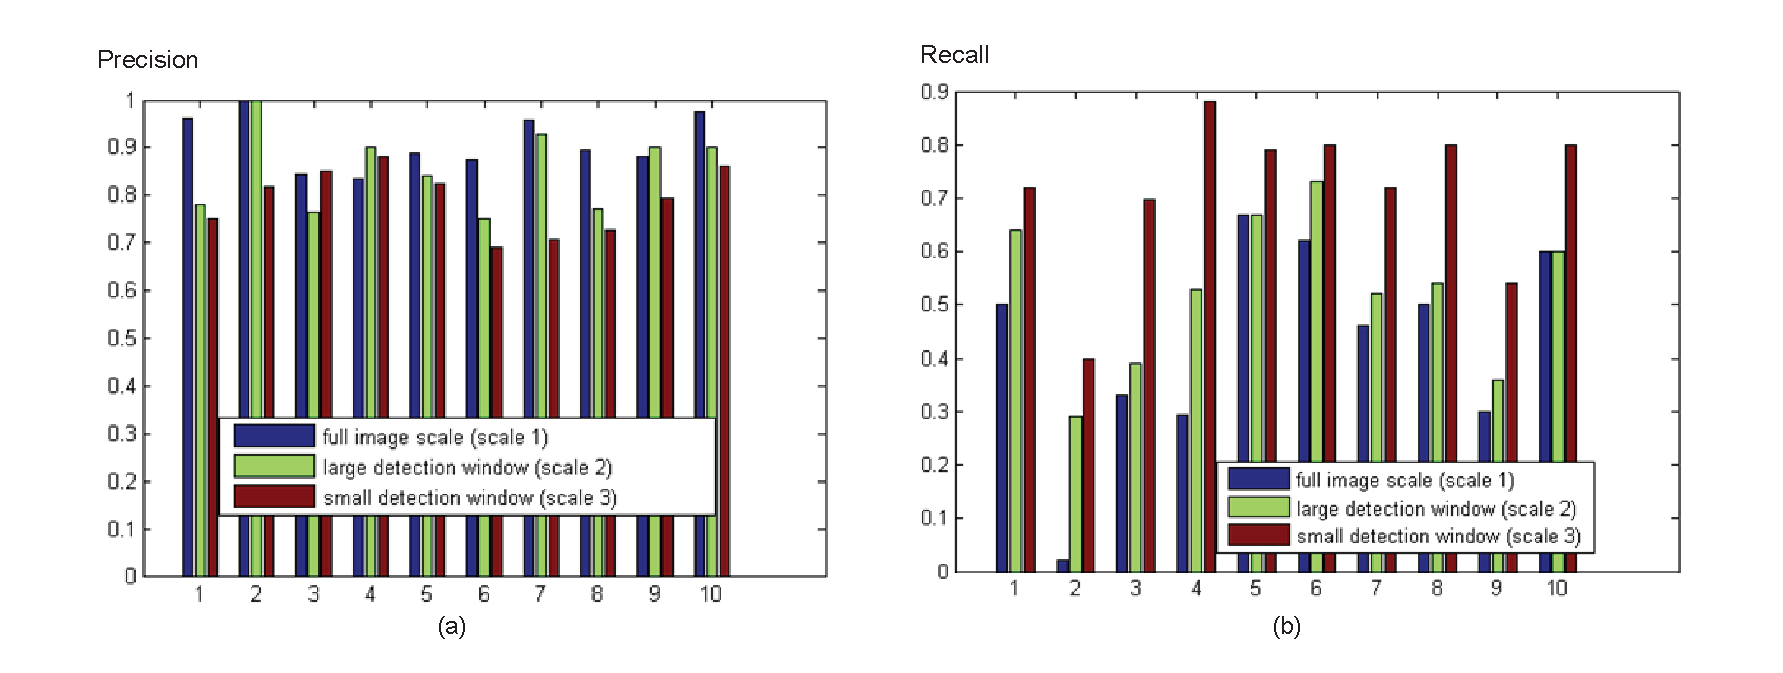
\includegraphics[width=\textwidth]{Chap2_trend}
\vspace {0em}\caption{(A) Trend for decreasing precision in finer scales. (B) Trend for increasing recall in finer scales.}
\label{Chap2_trend}
\vspace {0em}
\end{figure}



Table {\ref{earres}} and {\ref{mouthres}} show the results for ear and mouth/lip disease images. Our method achieved average precisions of
80.7\% and 84.2\%, while the baselines of test set quality were
43.4\% and 47.5\%, respectively. The three evaluation criteria in
table {\ref{earres}} are similar between the two methods ($p>0.1$), and the
average precision of our method for ear disease retrieval was
higher than that of the supervised method. In table \ref{mouthres}, our
method achieved around 6\% average higher precision than the
supervised method ($p=0.15$), at the cost of lower recall. One
possible reason is that the body parts in some mouth disease
images from the test sets are at very different angles and considerably
deformed.
\setlength{\tabcolsep}{5.7pt}
\begin{sidewaystable}
\centering
\caption{Performance Comparison on Ten Ear Disease Image Test Sets.}\label{earres}
\renewcommand{\arraystretch}{1.3}
\begin{tabular}{cccccccc}
\hline
\multicolumn{2}{l}{Ear diseases} & \multicolumn{3}{l}{Object Detection Based Method} &
\multicolumn{3}{l}{Supervised Classification Method} \\ \hline
Disease CUI    &Disease Term & Precision & Recall & F1    & Precision & Recall & F1 \\ \hline
C0008373	&Cholesteatoma&	0.794	&0.818&	0.806&	0.881&	0.953&	0.915\\ \hline
C0013446	&Acquired Ear Deformity&	1.000&	0.828&	0.906&	0.819&	0.863&	0.840\\ \hline
C0013449	&Ear Neoplasms	&0.875	&0.412&	0.560&	0.733	&0.567&	0.639\\ \hline
C0029877	&Ear Inflammation	&0.921&	0.778	&0.843	&0.822	&0.804	&0.813\\ \hline
C0154258	&Gouty tophi of ear	&0.792	&0.655&	0.717&	0.614	&0.470&	0.532\\ \hline
C0347354	&Benign neoplasm of ear	&0.571	&0.533&	0.552&	0.820	&0.497&	0.619\\ \hline
C0423576	&Irritation of ear	&0.733	&0.611	&0.667	&0.933	&0.607	&0.735\\ \hline
C0521833	&Bacterial ear infection&	0.786	&0.647&	0.710&	0.820	&0.670&	0.737\\ \hline
C0729545	&Fungal ear infection	&0.800	&0.696	&0.744&	0.728	&0.864	&0.791\\ \hline
C2350059	&Cancer of Ear&	0.800	&0.414&	0.545&	0.797	&0.699&	0.736\\ \hline
\multicolumn{2}{l}{Average}&0.807&	0.639	&0.705&	0.797	&0.699&	0.736\\ \hline
\end{tabular}
\end{sidewaystable}

\setlength{\tabcolsep}{5.7pt}
\begin{sidewaystable}
\centering
\caption{Performance Comparison on Ten Mouth/Lip Disease Image Test Sets.}\label{mouthres}
\renewcommand{\arraystretch}{1.3}
\begin{tabular}{cccccccc}
\hline
\multicolumn{2}{l}{Mouth/Lip diseases} & \multicolumn{3}{l}{Object Detection Based Method} &
\multicolumn{3}{l}{Supervised Classification Method} \\ \hline
Disease CUI    &Disease Term & Precision & Recall & F1    & Precision & Recall & F1 \\ \hline
C0007971	&Cheilitis	&0.846&	0.667&	0.746	&0.828&	0.893	&0.859\\ \hline
C0019345	&Herpes Labialis&0.900	&0.486	&0.632	&0.817	&0.953&	0.880\\ \hline
C0023761	&Lip Neoplasms	&0.909	&0.500	&0.645	&0.607	&0.553	&0.579\\ \hline
C0149637	&Carcinoma of lip	&0.952	&0.435	&0.597&	0.819	&0.906	&0.860\\ \hline
C0153932	&Benign neoplasm of the lip	&0.625	&0.333	&0.435	&0.833&	0.713	&0.769\\ \hline
C0158670	&Congenital fistula of lip	&0.700	&0.368&	0.483	&0.693	&0.800	&0.743\\ \hline
C0221264	&Cheilosis	&0.750	&0.577	&0.652	&0.813	&0.867	&0.839\\ \hline
C0267022	&Cellulitis of lip	&0.923	&0.600	&0.727	&0.810	&0.917	&0.860\\ \hline
C0267025	&Contact cheilitis	&0.950&	0.543	&0.691	&0.849	&0.943	&0.894\\ \hline
C0267032	&Granuloma of lip	&0.867	&0.500	&0.634&	0.721	&0.865&	0.786\\ \hline
\multicolumn{2}{l}{Average}&0.842	&0.501	&0.624&	0.779&	0.841	&0.807 \\ \hline
\end{tabular}
\end{sidewaystable}

\subsection{Multiple-organ disease classification}
Experiment B evaluated the performance of our method on 220
images of two diseases that are located on multiple organs.
Table {\ref{multiorgan}} shows that the precision of the proposed method on
both test sets was $>80\%$. Compared with the supervised
method, our method improved precision by more than 10\% in
these two cases. Since the proposed method is guided by the
semantic information of body part location, it can detect
various kinds of positive images, whereas the supervised method
does not make use of the high-level features that have greater
semantic meaning.

For hand, foot, and mouth disease, 42.9\%, 28.6\%, and
37.1\% of the positive images in the test set contained a hand,
foot, and mouth, respectively. A few positive images contained
two or three body parts at the same time. The hand, foot, and
lip/mouth detectors contributed to finding 28.6\%, 14.3\%, and
28.6\% of the total positive images. For Ascher's syndrome,
67.9\% and 32.1\% positive test images contained lip and eye,
respectively. The corresponding mouth/lip and eye detectors
found 57.1\% and 28.6\% positive images, respectively, from the
whole test sets.

In summary, we trained five organ detectors and reused them
to filter 2220 web images of 32 different diseases in two experiments.
Compared with the supervised approach that require
training 32 classifiers for each of the diseases, we reduce the
labeling efforts to 15.6\%. The average retrieval precision of our
method on all the 32 datasets was 81.6\%, an improvement of
3.9\% compared with the supervised method. For 13 out of 32
disease datasets, we improved the retrieval precision by 10\%.

\setlength{\tabcolsep}{5.7pt}
\begin{table*}
\centering
\caption{Performance Comparison on Ten Mouth/Lip Disease Image Test Sets.}\label{multiorgan}
\renewcommand{\arraystretch}{1.3}
\begin{tabular}{{lm{3.5cm}m{3.5cm}m{3.5cm}}}
\hline
\multicolumn{2}{l}{Disease CUI} & C001852 &C0339085 \\
\multicolumn{2}{l}{Disease Term} & Hand, Foot and Mouth Disease &Ascher's syndrome \\ \hline
%Positive percentage &0.58 &0.56
\multicolumn{2}{l}{Disease Locations} &C0222224  Skin structure of hand &C0023759 Lip structure\\
\multicolumn{2}{l}{ }&C0222289 Skin structure of foot  &C0015426 Eyelid structure\\
\multicolumn{2}{l}{ }&C0026639 Oral mucous membrane structure& \\
\multicolumn{2}{l}{Detectors} & Hand, Foot and Mouth/Lip &Mouth/Lip and Eye \\
\multicolumn{2}{l}{Positive percentage} & 0.58 &0.56 \\ \hline
\multirow{2}{*}{Precision} &Object detection based     & 0.8333 &0.8889\\
                        &Supervised classification  &0.6944  &0.7857\\
\multirow{2}{*}{Recall} &Object detection based     & 0.7143 &0.8571\\
                        &Supervised classification  &0.7753  &0.9429\\
\multirow{2}{*}{F1} &Object detection based     & 0.7692 &0.8727\\
                        &Supervised classification  &0.7326  &0.8571\\ \hline
\end{tabular}
\end{table*}




\section{Discussion}
With the aim of achieving large-scale medical image retrieval,
we compared the proposed ontology-guided approach with
standard supervised classification. We showed that the proposed
method achieves a precision comparable to that of the supervised
method while saving manual labeling efforts by an order
of magnitude. The results also illustrated that our method has
limitations in low recall values on some test sets and in decreasing
precision when the detection scale becomes smaller. To
improve the recall, we need more robust algorithms and better
data to train the organ detectors. For the limitation of decreasing
precision, we plan to build a two-layer learning model, in
which the first layer classifiers detect target objects at different
scales and the second layer classifier learns the weights to
combine results from the first layer and make final decisions.

The scale of our experiments is limited owing to the intensive
manual labeling work required for training data and evaluation
purposes. Our experiments are based on five organ detectors. In
the future, we plan to train more organ detectors and apply the
method to handle more diseases. We also found that a few
organs, such as skin, muscle, and veins, do not appear as concrete
objects in images. Our method based on object detection
is insufficient for diseases on these organs. In future work, we
plan to add texture pattern recognition to further improve the
retrieving precision and cover a wider range of diseases.

Our approach also depends on disease-organ relationships in
the UMLS, and assumes that the appearance of related organs
determines if the image is disease-related or not disease-related.
Although the assumption is true for many cases as we have
shown, a small number of false-positive samples retrieved by
our method are still non-disease images (only contain normal
organs), or images of a different disease. Another limitation of
this assumption is that the value of ``has\_finding\_site" relationship
in the UMLS is incomplete. Among 74 785 disease concepts
of semantic-type ``disease or syndrome," ``neoplastic
process," ``acquired abnormality," and ``congenital abnormality,"
44.1\% have values in ``has\_finding\_site." For disease terms that
have no body-site information, we plan to extend our approach
by scanning the web images with all organ detectors. In this
way, the ``has\_finding\_site" relationship in the UMLS can be
enriched by mining web images.

\section{Conclusions}
In this work, we developed an ontology-guided disease image
retrieval method based on body-part detection towards mining
web images to build a large-scale health image base for consumers.
Compared with standard supervised classification, the
proposed method improves the retrieval precision of complex
disease images by incorporating semantic information from
medical ontologies. In addition, our method significantly
reduces manual labeling efforts by reusing a set of pretrained
organ detectors. The resulting health image database is annotated
using terms from standard medical ontologies and will
create a rich source of information for multiple descriptive and
educational purposes. Although the scale of our study is limited,
it proves the concept that the web is a feasible source for
automatic health image retrieval, and it only requires a small
amount of manual effort to collect and annotate complex
disease images. In future work, we plan to improve the accuracy
of organ detectors and ontology-based classification, and extend
our approach to handle a wider range of diseases. 
%\input{chapters/content/chapter_3_NUMFL}
\chapter{Causal Inference Based Fault Localization for Numerical Software with Bayesian Additive Regression Trees}\label{chap:BART}


\section{Introduction}\label{BARTintro}
\vspace{-2pt}
With causal inference based SFL techniques\cite{bai2015numfl, baah2010causal, baah2011mitigating,shu2013mfl}, fault localization basically contains two steps: (1) controlling the confounding bias which is caused by confounding variables. (2) estimating the average failure causing effect of treatment variable $T$ on outcome $Y$. The second step, AFCE estimation, is a challenging because the functional form of the relationship between $T$ and $Y$ is unknown. In previous work, Baah et al’s used a parametric linear regression model to estimate a statement's AFCE. NUMFL used a quadratic regression model which a requires the user to pre-define the functional form of the dose-response function of the treatment $T$ (e.g. Figure 3.4). But if the parametric model is misspecified,, then AFCE estimation can be biased.

To solve the above problem in general settings, a non-parametric causal effect estimation model called Bayesian Additive Regression Trees (BART) has been proposed by Hill et al \cite{hill2012bayesian}. BART uses a sum-of-trees structure to approximate the dose-response function (DRF) of both the treatment variable and the confounding variables. 
Compared to methods such as NUMFL and Baah et al’s causal estimator, BART requires less guess-work in modeling dose-response functions.   

In this chapter, we proposal a new statistical fault localization method based on a BART model and evaluate it on numerical programs with single or multiple faults. The motivation for using BART in statistical fault localization is:
\vspace{-0.2cm}
\begin{itemize}
\item BART can flexibly fit non-linear response surfaces even with a large number of predictors
\item BART does not require the researcher to specify the functional form of the relationship between treatment and outcome. The user only needs to input the treatment, the confounding variables and the outcome, but does not need to specify how these variables are parametrically related. Also, unlike NUMFL, BART does not require a separate step to control confounding bias.
\item In an empirical study conducted by Hill et al., BART performed more effectively than propensity score matching based causal inference methods in average causal effect estimation for binary treatments. Hill et al also extended BART to detect nonlinear relationships between continuous treatments and outcomes. \cite{hill2012bayesian, hill2013assessing}.
\item Software is freely available and easy to use \cite{BARTMachine}.
\end{itemize}

The rest of the chapter is organized as follows: we present background on regression trees and the BART model in Section \ref{BARTbg}; using BART to estimate the failure-causing effect of a program expression is described in detail in Section \ref{BARTafce};  we report on ourempirical evaluation of this approach in Section \ref{BARTevaluation}; related work is surveyed in Section \ref{BARTrelatedwork}; and Section \ref{BARTconclusion} concludes the chapter.

\section{BART Model Algorithm}\label{BARTbg}%what is BART and why BART
The BART model algorithm consists of three parts: a sum of trees model, a regularization prior and a fitting algorithm, Markov Chain Monte Carlo (MCMC)
\subsection{Single Regression Tree Model}
A regression tree is one type of decision tree that predicts the value of a target variable based on several input variables \cite{loh2011classification}, and that handles continuous target variables. Figure \ref{singlergt} shows a single regression tree model. All the interior nodes of a regression tree have decision rules which send the input data set to either left or right side. After the input data set goes through the interior nodes and reaches the bottom of the tree, it is divided into several disjoint subgroups. Each group of data is represent by a leaf node.

\begin{figure*}[!thpb]
\centering
\includegraphics[width=0.5\textwidth]{chapter4_SingleRGT.pdf}
\caption{Single Regression Tree Structure}
\label{singlergt}
\end{figure*}

A single regression tree model is denoted as:
\begin{equation*}
Y=g(\pmb{Z}; R, M)+\epsilon
\end{equation*}
Here $\varepsilon  \sim N(0,{\sigma ^2})$ is a normally distributed error. $\pmb{Z}=[T,\pmb{X}]$ denotes all the variables related to the outcome $Y$, so $Z$ includes both treatment variable $T$ and confounding variables $\pmb{X}$. $R$ denotes a binary regression tree consisting a set of interior node decision rules and a set of terminal nodes, and $M=
{
 \mu _1, \mu _2, . . ., \mu _b
}$
denotes a set of parameter value associated with each of the $b$ terminal nodes of $R$. Each terminal node represent a regression model of outcome $Y$ on all the variables $Z$.

A regression tree model is often used in approximating unknown functions, such as the dose-response function of the treatment variable, $Y=f(T,\pmb{X})$. The regression tree model divides the value space of $[T,\pmb{X}]$ in to several subgroups with its tree structure and a regression model is fitted for each subgroup. When making an inference about $Y$ given values for the treatment and confounding variables $[T=t,\pmb{X}=\pmb{x}]$, the regression tree will first find out which subgroup the unit belongs to and then infer outcome $Y$ with the corresponding linear regression. A regression tree model has two advantages: (1) making predictions is fast and (2) it can handle non-linear function approximation.  The limitation of regression tree model is that a regression tree model may be an unstable decision tree. In other words, insignificant modification of the learning sample, such as eliminating several observations, could lead to radical changes in the tree structure: increase or decrease of tree complexity, or changes in splitting variables and values \cite{timofeev2004classification}.


\subsection{A sum-of-trees model}
BART is a sum-of-trees model. With the definition of a single tree model, the sum-of-trees model can be expressed as:
\begin{equation*}
Y = g(\pmb{Z};{R_1},{M_1}) + g(\pmb{Z};{R_1},{M_1}) +  \cdots  + g(\pmb{Z};{R_m},{M_m}) + \varepsilon
\end{equation*}
where each $(R_i,M_i)$ denotes a single sub-tree model and $\varepsilon  \sim N(0,{\sigma ^2})$.  $m$ denotes the number of trees in BART model. We have
 \begin{equation*}
 Y =f(\pmb{Z})=f(T,\pmb{X})= \left( {\sum\limits_{j = 1}^m {g(T,\pmb{X};{R_j},{M_j})} } \right) + \varepsilon
 \end{equation*}

Compared to single regression tree model, BART model has two advantages. First BART can incorporate interaction effects of varying orders. Unlike the single tree model, when $m>1$ the terminal node $\mu_i$ given by $g(\pmb{Z};{R_i},{M_i})$ is merely part of the conditional mean of $Y$ given $Z$. If the assignment of $\mu_i$ depends on just a single component of $Z$ (only one variable),  $\mu_i$  represents direct effect of that variable to $Y$. If the assignment of $\mu_i$ depends on more than one component of $Z$ (e.g., more than one variable), the terminal node will represent interaction effects of those variables. Because the BART model may be based on trees of varying sizes, the sum-of-trees structure can incorporate both direct effects and interaction effects of varying orders \cite{conference1997advances}. Second, fitting a BART model does not entail much more computation cost than fitting a large single tree model. This is because that BART can scale to large datasets using a parallel MCMC sampler \cite{pratola2014parallel, pratola2015bayesian}.  

\subsection{A regularization prior}
Fitting the BART model requires a prior distribution of all the parameters of the sum-of-trees model.  The prior regularizes the fit by keeping the individual tree's effect from being unduly influential. Without such a prior, large tree components would dominate the structure. The regularization prior can also help BART avoid overfitting. To simplify the prior specification, the trees in the BART model $(R_1, M_1), (R_2,M_2), \ldots, (R_m, M_m) $ are considered to be independent of each other and of $\sigma$. Also, the terminal node parameters $ \mu _{1j}, \mu _{2j}, . . ., \mu _{bj} $ of every tree $R_j$ are assumed to be independent. So we have:

\begin{equation*}
 \begin{array}{l}
P(({R_1},{M_1}),({R_2},{M_2}) \ldots ,({R_m},{M_m}),\sigma ) = \left[ {\prod\limits_j {P({R_j},{M_j})} } \right]p(\sigma )\\
\quad \quad \quad \quad \quad \quad \quad \quad \quad \quad \quad \quad \quad \quad \; = \left[ {\prod\limits_j {P({M_j}|{R_j})P({R_j})} } \right]p(\sigma )
\end{array}
 \end{equation*}
and
\begin{equation*}
P({M_j}|{R_j}) = \left[ {\prod\limits_i {P({\mu _{ij}}|{R_j})} } \right]
 \end{equation*}
Here ${\mu _{ij}} \in {M_j}$ denotes the $ith$ terminal node of the $jth$ regression tree. From the above equations, we can see that independence simplifies the problem of specifying the complete prior distribution to the specification of priors for just ${P({\mu _{ij}}|{R_j})}$, $P({R_j})$ and $P(\sigma)$. In reference \cite{chipman2010bart}, the specification of prior forms on $P(\sigma)$ is assumed to be an inverse chi-square distribution. The prior on ${P({\mu _{ij}}|{R_j})}$ is assumed to be a conjugate normal distribution. The prior on $P(R_j)$ is complex. It contains three aspects:
\begin{enumerate}
\item the probability that a node at depth $d$ is nonterminal, given by
\begin{equation*}
\alpha {(1 + d)^{ - \beta }},\quad \alpha  \in (0,1),\beta  \in [0,\infty )
 \end{equation*}
where $d$ is the number of edges from the node to the tree's root node. $\alpha {(1 + d)^{ - \beta }}$ is a decreasing function of $d$, making deeper nodes less likely to split. In other words, this prior specification puts higher probability on the trees whose terminal nodes do not vary too much in depth.
\item the prior probability that a variable is selected as the splitting variable at an interior node is $1/k$ and $k$ is the total number of variables including both treatment and confounders.
\item the prior probability that a splitting variable is split at a specific value $x$ is $1/N$, and $N$ is the total number of observed values of the splitting variable in the sample data set.
\end{enumerate}
The details of the prior specification for ${P({\mu _{ij}}|{R_j})}$, $P({R_j})$ and $P(\sigma)$ can be found in reference \cite{chipman2010bart}.


\subsection{Bayesian Backfitting MCMC Algorithm}
BART uses an iterative Bayesian backfitting  MCMC algorithm to fit the model \cite{gilks2005markov}. The algorithm uses Gibbs sampler \cite{casella1992explaining}. The Gibbs sampler makes $m$ successive draws of $(R_j, M_j)$ conditionally on $(R_{(j)}, M_{(j)}, \sigma)$:

\begin{equation*}
(R_j,M_j)|R_{(j)}, M_{(j)}, \sigma, Y
\end{equation*}
$j=1 \ldots m$, followed by a draw of $\sigma$ from the full conditional:

\begin{equation*}
\sigma |{R_1}, \ldots ,{R_m},{M_1}, \ldots ,{M_m},Y
\end{equation*}
Here $R_{(j)}$ represents all the trees except $R_j$, so $R_{(j)}$ will be a set of $m-1$ trees. $M_{(j)}$ is similarly defined as $R_{(j)}$.

\section{AFCE Estimation With BART}\label{BARTafce}% how to use BART

In this section, we introduce our approach to using BART to estimate the AFCE of a numerical program expression, which is adapted from Hill et al. \cite{hill2012bayesian}. Hill et al. have proved that BART is effective in average causal effect estimation when the treatment variable is binary. In \cite{hill2012bayesian}, the causal effect of a binary treatment variable $T$ for individual $i$ is defined as $Y_i(1)-Y_i(0)$. $Y_i(1)$ and $Y_i(0)$ are the {\it potential outcomes} for individual $i$, which means the outcomes that would be observed under $T=0$ and $T=1$. Since $Y_i(1)$ and $Y_i(0)$ cannot be both observed fro any individual in the observational study, the causal effect is measured by the average causal effect $E[Y(1)-Y(0)]$.  Based on the potential outcome notation, we briefly review Hill’s algorithm:

Hill et al. use BART to estimate average causal effects such as $E[Y(1)|\pmb{X}=\pmb{x}] - E[Y(0)|\pmb{X}=\pmb{x}]=E[Y|T=1, \pmb{X}=\pmb{x}]-E[Y|T=0, \pmb{X}=\pmb{x}]=f(1,\pmb{x})-f(0,\pmb{x})$ . $f(t,\pmb{x})$ is the function that predicts the outcome $Y$ using the values of both treatment variable and confounding variables.  The algorithm contains the following steps:
\begin{enumerate}
\item Fit a BART model with the MCMC algorithm to the full sample.
\item Generate a posterior prediction for each unit by setting the treatment variable value to $T=1$ and keep the confounding variable values unchanged.
\item Generate a posterior prediction for each unit by setting the treatment variable value to $T=0$ and keep the confounding variable values unchanged.
\item Calculate the difference between the posterior predictions for each unit.
\item Estimate the average causal effect by averaging all the differences of posterior predictions.
\end{enumerate}

In step 1, the fitted BART model characterizes the causal relationship between treatment $T$ and outcome $Y$ given the confounders $\pmb{X}$. We can use the fitted model to predict the outcome $Y$ under different $(T, \pmb{X})$ conditions. For an untreated unit $(T=0, \pmb{X}=\pmb{x})$,  if we set the treatment variable to 1 and then input $(T=1, \pmb{X}=\pmb{x})$ into the BART model, the output is the estimated potential outcome $Y(1)$ for that unit in treated condition. Similarly, we can estimate the potential outcome $Y(0)$ of a treated unit in untreated condition by inputting $(T=0, \pmb{X}=\pmb{x})$ into the BART model. Thus, in steps 2 and 3, BART is used to predict the missing potential outcomes (counterfactual outcomes). Thus, the difference calculated in step 4 is the individual (unit) level causal effect. The average of these differences is average causal effect, which is estimated in the step 5.

If the treatment variable is continuous,  we can use BART to approximate the dose-response function $Y=f(T,\pmb{X})$ of the continuous treatment $T$ and confounding variables $\pmb{X}$.  As we mentioned before, the BART model does not require the user to make assumptions or specify the functional form of the dose-response function.  But AFCE estimation for numerical expressions with BART is challenging. In previous CSFL methods (e.g. NUMFL or Baah et al’s causal estimator), the average failure-causing effect can be characterized by the coefficient of a regression model.  But with the BART model, each tree $g(\pmb{Z};{R_1},{M_1})$ only explains part of $Y$, so there are no parameters in BART that can directly characterize the AFCE. 

To solve this problem, we proposed a novel BART-based average causal effect estimation algorithm for continuous treatment. We first estimate the individual-level causal effect for  each unit in the sample. Then the average value of the estimated individual-level causal effects in the data set is the estimated AFCE of the expression.  Assume the unit $i$ has treatment value $T=t$ and confounder values $\pmb {X}=\pmb {x}$. We can use the fitted BART model to estimate the outcome for the unit $y=f(t,\pmb{x})$. Then we increase the treatment value to $t'=t+\varepsilon$, where $\varepsilon $ is a small number. We input $t'$ and $\pmb{x}$ into the fitted BART model and get the estimated posterior values $y'=f(t',\pmb{x})$. Then the estimated causal effect of $T$ on $Y$ for unit $i$ is $\left| {y - y'} \right|$. The algorithm is as follows:
\begin{enumerate}
\item Fit a BART model to the full sample using the MCMC algorithm.
\item Given a unit in the observational data set, we input its treatment and confounder values into the fitted BART model. 
\item Increase the value of the treatment variable from $t$ to $t'=t+\varepsilon$, but keep the confounding variables unchanged. The causal effect of treatment for this unit is estimated by the change in the output of the BART model, $|f(t',\pmb{x})-f(t,\pmb{x})|$.
\item Repeat step 2 and step 3 for all the units in the dataset.
\item Estimate failure-causing effect by averaging all the differences of posterior predictions.
\end{enumerate}

In the above algorithm, the BART model fitted in step 1 is used to approximate the DRF $Y=f(T,\pmb{X})$. Step 2 and step 3 estimate the treatment causal effect for a given sample unit. Step 4 and step 5 estimate the average failure-causing effect of the treatment on the outcome.

One problem in step 3 is how to choose the value of the small number $\varepsilon $. Because treatment variables in different numerical expressions have different scales of values, it is hard to find a constant $\varepsilon$ which can make $t+\varepsilon$ be a reasonable value for all the treatments. To address this problem, we use the method illustrated by Figure \ref{bartace}.  The original sample data set is shown in Figure \ref{bartace} (a).  We sort the original sample data set in increasing order according to the value of the treatment variables. The sorted data set is shown in Figure \ref{bartace} (b). The increased treatment variable value $t'$ in step 3 is equal to the treatment variable value $t$ of the next unit in the sorted data set, and the last unit in the list will be discarded. Thus,  for a data set with $n$ observational units, we will have a new data set of $n-1$ units after increasing the treatment variable. The new data set is shown in Figure \ref{bartace} (c). In this method, the value of $t'=t+\varepsilon$ and the value of $t$ are likely to be in the same scale, because they are neighbor in the sorted data set. 

\begin{figure*}[!thpb]
\centering
\includegraphics[width=1\textwidth]{chapter4_BART_ACE.pdf}
\caption{EXAMPLE OF TREATMENT VARIABLE INCREASE}
\label{bartace}
\end{figure*}

\section{EMPIRICAL EVALUATION}\label{BARTevaluation}% result

To evaluate the effectiveness of BART model, we conducted an empirical study on the same subject programs described in chapter 3.  The test suite is also identical to the test suite in section \ref{numfl_evaluation}.  Overall, there wre 92 faulty subject-programs versions with a single fault and 25 faulty subject-program versions with two faults. Ochiai, Dstar, SOBER, ESP-SIV and ESP-SCP were used as the base line techniques to be compared with BART model. We also compared the performance of the BART model with NUMFL-GPS and NUMFL-CBPS, which are described in chapter 3. We measured the costs of applying BART and the other metrics by the percentage of {\it subexpressions} that need to be examined, in decreasing order of suspiciousness scores, to find the fault, assuming the fault is recognized when it is encountered.

In the study, we used R package "BARTMachine" \cite{BARTMachine} to fit the BART model. We tried 10 trees and 50 trees in the sum-of-trees structure.  The BART model is fitted with both passing and failing tests. The number tests for each subject program ranged from 3000 to 8000 as shown in Table \ref{subpro}. To analyze the sensitivity of the BART model to the number of  tests, we also tried to train BART model with fewer data (300 tests). The sensitivity of the BART model to the number of trees and the number of tests are discussed in section \ref{BARTsensitivity}.

\subsection{Comparative Performance of BART vs. Baselines}

Figure \ref{BART_VS_Base} shows the results of comparisons of BART with each of the baseline metrics.  In each graph, the vertical axis represents the percentage improvement (reduction) in cost. The horizontal-axis represents different subject-program versions for which there are cost differences between the metrics, with each version represented by a vertical bar.   Bars above the zero-line represent versions for which BART performed better than the baseline metric and bars below zero represent versions for which BART performed worse.  The length of each bar represents the magnitude of the corresponding cost difference.

\textit{\textbf{ BART vs. Ochiai.}}  Over all 92 faulty subject-program versions, BART performed better than the Ochiai metric on 75 versions but BART performed worse on 17 versions.  There were 41 versions for which BART performed at least 20\% better than the Ochiai metric.  There were just 4 versions for which the latter performed better than BART.

\textit{\textbf{ BART vs. DStar.}}  BART performed better than DStar on 77 subject-program versions but BART performed worse than DStar on 15 versions.  BART performed at least 20\% better than DStar on 44 versions, whereas DStar performed at least 20\% better than BART on just 4 versions.

\textit{\textbf{ BART vs. ESP-SIV.}} BART performed better than ESP-SIV on 78 subject-program versions but BART performed worse than ESP-SIV on 14 versions.  BART performed at least 20\% better than ESP-SIV on 30 versions, whereas ESP-SIV never performed at least 20\% better than BART.

\textit{\textbf{ BART vs. ESP-SCP.}}  BART performed better than ESP-SCP on 75 subject-program versions but BART performed worse than ESP-SCP on 17 versions.  BART performed at least 20\% better than ESP-SIV on 22 versions, whereas ESP-SCP performed at least 20\% better than BART on just 2 versions.

\textit{\textbf{ BART vs. SOBER.}}  BART performed better than SOBER on 73 subject-program versions but BART performed worse than SOBER on 19 versions.  BART performed at least 20\% better than SOBER on 39 versions, whereas SOBER performed at least 20\% better than BART on just 5 versions.

\begin{sidewaysfigure}
\centering
\includegraphics[width=\textwidth]{chapter4_BART_VS_Base.pdf}
\caption{Performance of BART relative to baseline metrics on individual single-fault program versions.}
\label{BART_VS_Base}
\end{sidewaysfigure}

Figure \ref{BART_VS_Base_M} contrasts the performance of BART on the individual two-fault program versions with that of the baseline metrics.  Over all 25 faulty subject-program versions, BART performed better than SOBER on 19 versions but performed worse on 6 versions.  There were 8 versions for which BART performed at least 10\% better than SOBER but 3 versions for which SOBER performed at least 10\% better than BART.  Ochiai performed better than BART on 5 versions but performed worse on 20 versions. BART performed at least 10\% better than Ochiai on 13 versions. BART performed better than both ESP-SIV and ESP-SCP on 20 versions.   BART performed better than DStar on 19 versions.

\begin{sidewaysfigure}
\centering
\includegraphics[width=\textwidth]{chapter4_BARTvsBase_M.pdf}
\caption{Performance of BART relative to baseline metrics on individual two-faults program versions.}
\label{BART_VS_Base_M}
\end{sidewaysfigure}


\subsection{BART Model vs NUMFL}
Table \ref{tableBARTvsNUMFL} shows the average percentage of subexpressions that had to be examined to find the fault, computed across all the faulty versions, for the BART model and NUMFL.  Because QRM is proved to have better performance than DLRM in chapter 3, here we only show the results of NUMFL-GPS-QRM and NUMFL-CBPS-QRM.  From Table \ref{tableBARTvsNUMFL}, there were 11 subject programs for which BART performed better than NUMFL-GPS-QRM. There were 5 subject programs for which NUMFL-GPS-QRM performed better than BART. BART performed better than NUMFL-CBPS-QRM on 14 subject programs. There were only 2 subject programs for which NUMFL-CBPS-QRM performed better than BART.

Figure \ref{BARTvsQRM} graphically contrasts the performance of BART and NUMFL-GPS-QRM on the single fault versions.  BART performed better than NUMFL-GPS-QRM on 54 versions, while NUMFL-GPS-QRM performed better on 38 versions.  BART performed at least 20\% better than NUMFL-GPS-QRM on 9 versions, whereas NUMFL-GPS-QRM performed at least 20\% better than BART on 6 versions. Figure \ref{BARTvsCBPS} graphically contrasts the performance of BART and NUMFL-CBPS-QRM on the single fault versions.  BART performed better than NUMFL-CBPS-QRM on 61 versions, while NUMFL-CBPS-QRM performed better on 31 versions.  BART performed at least 20\% better than NUMFL-CBPS-QRM on 17 versions, whereas NUMFL-CBPS-QRM performed at least 20\% better than BART on just 4 versions.

In summary, BART  performed better than both NUMFL-GPS-QRM and NUMFL-CBPS-QRM on single-fault programs. This suggests that BART model can well approximate the DRF of treatment variable and confounding variables.

\begin{table*}[htbp!]
\caption{AVERAGE FAULT LOCALIZATION COSTS OF BART AND NUMFL METRICS ON SINGLE-FAULT PROGRAM VERSIONS}
\label{tableBARTvsNUMFL}
\centering
      \begin{tabular}{|l|c|c|c|}
      \hline
\multirow{2}{*}{Subject Program}	& \multirow{2}{*}{BART}&	\multicolumn{2}{|c|}{{\bf NUMFL}}	\\	\cline{3-4}
& & GPS-QRM	&CBPS-QRM \\ \hline
Apache\_EigenDecompose &	2.50\%&	12.3\%	&	8.8\%	\\	\hline
Apache\_DScompiler&	9.72\%&	11\%	&	12\%	\\	\hline
Apache\_BigMatrix	&	9.00\%&11.4\%	&	9.9\%	\\	\hline
Apache\_Rotation3D&	9.07\%&	8\%	&	18.9\%	\\	\hline
Ojaljo\_SchurDecompose&	10.61\%&	11.4\%	&	14\%	\\	\hline
Jama\_MatrixDecompose	&11.62\%&	14.2\%	&	23\%	\\	\hline
SciMark\_LU&8.33	\%&	15.3\%	&	27.8\%	\\	\hline
SciMart\_FFT&	 27.59\%&	9.5\%	&	19.8\%	\\	\hline
Apache\_SymmLQ&	 1.75\%&	2.6\%	&	4.4\%	\\	\hline
Apache\_SplineInterpolator&	 37.78\%&	31.7\%	&	35\%	\\	\hline
Apche\_SimpleRegress&	 1.70\%&	4.3\%	&	17\%	\\	\hline
Apache\_SchurTransformer&	 4.56\%&	3.3\%	&	14.9\%	\\	\hline
Apache\_MillerUpdatRegress&	 1.24\%&	7.5\%	&	9.9\%	\\	\hline
Apache\_HarmonicFitter&	30.10\%&	27.3\%	&	32\%	\\	\hline
Apache\_FastSine&	1.53\%&	1.5\%	&	13\%	\\	\hline
Apache\_FastCosine	&1.29	\%&1.3\%	&	1.2\%	\\	\hline
Average Cost	&	10.52\%&10.8\%	&	16.4\%	\\	\hline
\end{tabular}
\end{table*}

\begin{figure*}[!thpb]
\centering
\includegraphics[width=0.8\textwidth]{chapter4_BARTvsGPS_QRM.pdf}
\caption{Relative performance of BART and NUMFL-GPS-QRM on individual single-fault program versions.}
\label{BARTvsQRM}
\end{figure*}

\begin{figure*}[!thpb]
\centering
\includegraphics[width=0.8\textwidth]{chapter4_BARTvsCBPS.pdf}
\caption{Relative performance of NUMFL-CBPS-QRM on individual single-fault program versions.}
\label{BARTvsCBPS}
\end{figure*}

Table \ref{tableBARTvsNUMFL_M} shows the average cost, over the faulty versions of each subject program into which two-fault were injected, of localizing the first fault to be found, for both BART and NUMFL.  From Table \ref{tableBARTvsNUMFL_M}, BART and NUMFL-GPS-QRM have similar performance on two faults subject programs. BART performed better than NUMFL-GPS-QRM on the versions of  2 subject programs, but performed worse than NUMFL-GPS-QRM on the versions of 3 subject program.  BART performed better than NUMFL-CBPS-QRM on the versions of 4 subject programs, but performed worse than NUMFL-CBPS-QRM on the versions of only 1 subject program.

Figure \ref{BARTvsGPS_M} graphically contrasts the performance of the BART and NUMFL-GPS-QRM on the individual two-fault versions.  BART performed better than NUMFL-GPS-QRM on 13 versions and BART performed worse on 12 versions.  BART performed at least 10\% better than NUMFL-GPS-QRM on 7 versions, whereas NUMFL-GPS-QRM performed at least 10\% better than BART on just 1 version. Figure \ref{BARTvsCBPS_M} graphically contrasts the performance of the BART and NUMFL-CBPS-QRM on the individual two-fault versions.  BART performed better than NUMFL-CBPS-QRM on 13 versions and BART performed worse on 12 versions.  BART performed at least 10\% better than NUMFL-CBPS-QRM on 7 versions, whereas NUMFL-CBPS-QRM performed at least 10\% better than BART on just 1 version.

\begin{table*}[htbp!]
\caption{AVERAGE FAULT LOCALIZATION COSTS OF BART AND NUMFL ON TWO-FAULT PROGRAM VERSIONS}
\label{tableBARTvsNUMFL_M}
\centering
      \begin{tabular}{|l|c|c|c|}
      \hline
\multirow{2}{*}{Subject Program}	& \multirow{2}{*}{BART}&	\multicolumn{2}{|c|}{{\bf NUMFL}}	\\	\cline{3-4}
& & GPS-QRM	&CBPS-QRM \\ \hline
Apache\_EigenDecompose	&7.98	\%&10.3\%	&	11.1\%	\\	\hline
Apache\_DScompiler	&	5.13\%&4.5\%	&	5.9\%	\\	\hline
Apache\_Rotation3D	&	10.69\%&7.0\%	&	3.0\%	\\	\hline
Ojaljo\_SchurDecompose	&17.55	\%&5.4\%	&	19.8\%	\\	\hline
Jama\_MatrixDecompose	&	4.65\%&14.1\%	&	23.4\%	\\	\hline
{\bf Average Cost} &9.20\% &8.26\% &12.64\%\\ \hline
\end{tabular}
\end{table*}

\begin{figure*}[!thpb]
\centering
\includegraphics[width=0.8\textwidth]{chapter4_BARTvsGPS_QRM_M.pdf}
\caption{Relative performance of BART and NUMFL-GPS-QRM on two-fault program versions.}
\label{BARTvsGPS_M}
\end{figure*}

\begin{figure*}[!thpb]
\centering
\includegraphics[width=0.8\textwidth]{chapter4_BARTvsCBPS_M.pdf}
\caption{Relative performance of BART and NUMFL-CBPS-QRM on two-fault program versions..}
\label{BARTvsCBPS_M}
\end{figure*}

\subsection{Sensitivity of BART model on the number of trees and  the number of tests}\label{BARTsensitivity}

In previous sections, we used the data from all tests to fit a BART model with 10 trees in the sum-of-trees structure. In this section, we examine whether if increasing number of trees or decreasing the number of tests would influence the performance of BART. In Table \ref{sensitivity}, the first column is the fault localization cost of the BART model containing 10 trees, and fitted with 3000 tests. The second column is the fault localization cost of the BART model containing 50 trees, and fitted with 3000 tests. The third column is the fault localization cost of the BART model containing 10 trees, but fitted with only 300 tests. From Table \ref{sensitivity}, it can be seen that when we increased the number of trees from 10 to 50, the BART model has better performance on 6 subject programs. But there are also 6 subject program where the BART model's performance became worse after the number of trees was increased. The average cost across 16 subject programs is roughly same: 10.52\% for the BART model with 10 trees and 10.58\% for the BART model with 50 trees. This suggests that 10 trees are enough to handle the nonlinearity problem in AFCE estimation at least with programs that are similar to those used in the study.  When we decrease the number of tests to 300, the average cost is slightly increased to 10.74\%.  This means that the BART model does not require a large number of tests to localize faults in numerical softwares.

\begin{table*}[htbp!]
\caption{AVERAGE FAULT LOCALIZATION COSTS OF BART MODEL WITH DIFFERENT NUMBER OF TREES AND DIFFERENT NUMBER OF TESTS ON SINGLE-FAULT PROGRAM VERSIONS }
\label{sensitivity}
\centering
      \begin{tabular}{|l|c|c|c|}
      \hline
\multirow{2}{*}{{\bf Subject Program}}	&	\multicolumn{3}{|c|}{{\bf BART Model}}	\\	\cline{2-4}
& 10 trees & 50 trees & 300 tests\\ \hline
Apache\_EigenDecompose			&	2.50	\%	&	3.07	\%	&	2.38	\%	\\ \hline
Apache\_DScompiler			&	9.72	\%	&	8.61	\%	&	9.64	\%	\\ \hline
Apache\_BigMatrix			&	9.00	\%	&	9.05	\%	&	9.00	\%	\\ \hline
Apache\_Rotation3D			&	9.07	\%	&	8.73	\%	&	8.16	\%	\\ \hline
Ojaljo\_SchurDecompose			&	10.61	\%	&	9.89	\%	&	11.44	\%	\\ \hline
Jama\_MatrixDecompose			&	11.62	\%	&	11.16	\%	&	11.32	\%	\\ \hline
SciMark\_LU			&	8.33 \%	&	9.72	\%	&	6.94	\%	\\ \hline
SciMart\_FFT			&	27.59	\%	&	26.72	\%	&	27.59	\%	\\ \hline
Apache\_SymmLQ			&	1.75	\%	&	1.75	\%	&	1.75	\%	\\ \hline
Apache\_SplineInterpolator			&	37.78	\%	&	40	\%	&	45.56	\%	\\ \hline
Apche\_SimpleRegress			&	1.70	\%	&	1.70	\%	&	1.70	\%	\\ \hline
Apache\_SchurTransformer			&	4.56	\%	&	4.88	\%	&	4.23	\%	\\ \hline
Apache\_MillerUpdatRegress			&	1.24	\%	&	1.24	\%	&	1.24	\%	\\ \hline
Apache\_HarmonicFitter			&	30.10	\%	&	30.08	\%	&	28.06	\%	\\ \hline
Apache\_FastSine			&	1.53	\%	&	1.53	\%	&	1.53	\%	\\ \hline
Apache\_FastCosine			&	1.29	\%	&	1.29	\%	&	1.29	\%	\\ \hline
Average Cost 	&	10.52\% 	&10.58\% 	&10.74\%	\\ \hline
\end{tabular}
\end{table*}

\subsection{Computation Time Analysis}
In this study, we used a Dell Precision T5600 with two 2.30 GHz Intel Xeon CPUs and 64 GB RAM. Table \ref{BARTcomputetime} summarized the average computation time of the three BART models described in last section on each subject program.  When the number of trees increased from 10 to 50, the average computation cost nearly doubled. If we reduced number the tests from more than 3000 to 300, the computation cost was reduced more than 50\%.  From Table \ref{BARTcomputetime} and Table \ref{sensitivity}, we can conclude that the BART model with 10 trees and fitted with 300 tests had the best cost-performance ratio among the three BART models fitted with different settings. But we also need to point out that even when the BART model is fitted with 300 tests, its computation cost is still about twice of the computation cost of NUMFL. Thus, computation cost is a weakness of applying BART on localizing faults in numerical softwares. 

\begin{table*}[htbp!]
\caption{AVERAGE COMPUTATION TIME OF BART ON SINGLE-FAULT PROGRAM VERSIONS }
\label{BARTcomputetime}
\centering
      \begin{tabular}{|l|c|c|c|}
      \hline
\multirow{2}{*}{{\bf Subject Program}}	&	\multicolumn{3}{|c|}{Average Computation Time (Secs)}	\\	\cline{2-4}
& 10 trees & 50 trees & 300 tests\\ \hline

Apache\_EigenDecompose	&	2856.73	&	5530.20	&	1205.97	\\ \hline
Apache\_DScompiler	&	628.31	&	1243.78	&	274.88	\\ \hline
Apache\_BigMatrix	&	696.58	&	1337.73	&	292.28	\\ \hline
Apache\_Rotation3D	&	2668.41	&	5550.45	&	1082.64	\\ \hline
Ojaljo\_SchurDecompose	&	2636.96	&	5013.37	&	1313.53	\\ \hline
Jama\_MatrixDecompose	&	3134.49	&	6005.71	&	1262.88	\\ \hline
SciMark\_LU	&	167.94	&	332.45	&	121.38	\\ \hline
SciMart\_FFT	&	393.26	&	842.31	&	234.09	\\ \hline
Apache\_SymmLQ	&	908.12	&	1986.32	&	245.21	\\ \hline
Apache\_SplineInterpolator	&	364.80	&	747.42	&	135.00	\\ \hline
Apche\_SimpleRegress	&	823.34	&	1685.88	&	227.27	\\ \hline
Apache\_SchurTransformer	&	768.44	&	1539.44	&	315.65	\\ \hline
Apache\_MillerUpdatRegress	&	396.10	&	808.59	&	198.61	\\ \hline
Apache\_HarmonicFitter	&	326.09	&	673.73	&	120.28	\\ \hline
Apache\_FastSine	&	1006.86	&	2064.98	&	259.78	\\ \hline
Apache\_FastCosine	&	1089.13	&	2229.39	&	294.56	\\ \hline
\end{tabular}
\end{table*}

\section{RELATED WORK}\label{BARTrelatedwork}
The most related works to this study are those using BART model to estimate treatment causal effect. Hill et al. proposed to apply BART model for causal inference and data science \cite{hill2012bayesian, hill2013assessing}. In the paper, they designed the method of using BART to estimate average causal effect of binary treatment variable and discussed how to use BART to handle continuous treatment variables and outcome missing data. Later, Green et al. applied BART to model heterogeneous treatment effects \cite{green2012modeling}. Sparapani et al. extends the usefulness of BART in medical applications by addressing needs arising in survival analysis \cite{sparapani2016nonparametric}.

Another related work is using tree structure in fault localization. Chen et al \cite{chen2004failure} present a decision tree learning approach to identify the causes of failures in internet sites. Francis et al \cite{francis2004tree} use tree based method to classify software failures. Kiciman et al \cite{kiciman2005root} use decision tree to diagnose which component of large scale systems is the root cause of failure. However, unlike our models, all their works do not localize the fault on statement level.

\section{CONCLUSION}\label{BARTconclusion}
The BART model is a Bayesian non-parametric model which can capture both nonlinearities and interactions between variables without knowing how these variables are parametrically related . BART uses a sum of trees structure to approximate the dose-response function of continuous treatment variables. The AFCE can be estimated by averaging the predicted causal effect of treatment on the outcome at each observation unit. We reported the result of an empirical comparison of BART model with several competing fault localization metrics on both single-fault subject programs and multiple-fault subject programs. The BART model performed significantly better than the other techniques. We also compare the BART model with NUMFL, which was introduced in chapter 3. The result shows BART model outperformed NUMFL on single-fault programs. With multiple-fault programs, BART and NUMFL had similar performances.  We also study the sensitivity of the BART model to the number of trees and the number of tests. The results show BART is robust on the sample size and number of trees.   
%\chapter{Studying disease comorbidity network to detect genetic evidences for disease links: application on colorectal cancer and obesity}\label{cancer}

\section{Motivation}

A number of epidemiological studies suggest that
obesity increases the risk of colorectal cancer (CRC)
\cite{calle2003overweight,bardou2013obesity,khaodhiar1999obesity}.
Based on these evidences of co-occurrence,
many genetic factors have been proposed to explain the role of obesity in the development of CRC.
For example, both animal and human studies have demonstrated that the
increased release of insulin and reduced insulin signaling play roles
in obesity and colorectal carcinogenesis \cite{pollak2008insulin,leroith2003insulin,renehan2004insulin}.
Experiments also show that obesity leads to altered level of adipocytokines,
such as Adiponectin \cite{dalamaga2012role,an2012adiponectin,wei2005low}
and leptin \cite{stattin2003plasma,tamakoshi2004leptin}, which may either prevent or foster carcinogenesis.

The mechanism for the association between obesity and CRC is multifactorial and inconclusive
\cite{khaodhiar1999obesity,danese2012role}. Shared comorbidities between
obesity and CRC can provide unique insights into the common genetic basis for the two diseases.
For example, type 2 diabetes is highly correlated with obesity and was identified as a risk factor
for CRC \cite{berster2008type}. A few studies then discovered that genetic factors
of insulin resistance, which occur in type 2 diabetes, contribute in explaining the role of obesity
in CRC \cite{komninou2003insulin}. However, both obesity and CRC are heterogeneous conditions.
Over 40\% of the obese population is not characterized by the presence of insulin
resistance \cite{mesquita2009metabolically}. We hypothesize that systems approaches
to studying the diseases that are phenotypically-significant to
both CRC and obesity may offer new insights into the
common molecular mechanisms between the two interconnected diseases.

Systematic comorbidity studies have been conducted previously,
but mostly focused on pairwise comorbidities and their genetic overlaps.
Rhetsky et al. developed a statistical model to estimate the co-occurrence
relationship for each pair of 160 diseases \cite{rzhetsky2007probing},
and demonstrated that comorbidities are genetically linked. Park et al. \cite{park2009impact}
and Hidalgo et al. \cite{hidalgo2009dynamic}
detected the comorbidities pairs from the Medicare claims
(which only contain senior patients ages 65 or older) with statistical measures.
Roque et al. mined pairwise disease correlations using similar measures from
medical records of a psychiatric hospital \cite{roque2011using}.


In this study, we developed a novel approach to detect diseases
that have strong connections with both obesity and CRC in a comorbidity network.
Specifically, we first mined disease comorbidity relationships from a new data source and constructed
a novel disease comorbidity network. Then we extracted the local network consisting of all the
paths between obesity and CRC, and prioritized the nodes (diseases) that play critical roles
in maintaining the connection between the two diseases (Fig.\ref{crchypothesis}). Substantial literature evidences can support that the top ranked diseases have associations with both obesity and CRC. We investigated the gene expression profiles of a prioritized comorbid disease to facilitate detecting novel genetic basis underlying the link between obesity and CRC. Our approach is generalizable to study the genetic basis for other disease associations.
\begin{figure}[!tpb]
\vspace{-.1cm}
\centerline{\includegraphics[width=0.5\textwidth]{Chap5_crc_hypothesis.eps}}
%\vspace{-5cm}
\caption{Approach to detect the diseases that have strong connections with both obesity and CRC in the comorbidity network. Nodes D1, D2 and D3 were prioritized because they play important roles in maintaining the network structure and the connection. }
\vspace{-0cm}
\label{crchypothesis}
\end{figure}

\section{Data and methods}
Fig.\ref{crcmethod} shows the steps of our approach.
We first mined disease comorbidity relationships from large amounts of patient records
in a public database and constructed a disease comorbidity network.
We then extracted the local comorbidity cluster for obesity and CRC
and prioritize the candidate comorbidity that plays a critical role in connecting the two diseases.
Finally we conducted gene expression meta-analysis to
identify common genes shared by obesity, CRC and the prioritized comorbidity.
\begin{figure}[!tpb]
\vspace{-.1cm}
\centerline{\includegraphics[width=1\textwidth]{Chap5_crc_method.eps}}
%\vspace{-5cm}
\caption{Our approach contains three steps: (1) We constructed a comorbidity network based on data mining; (2) we extracted the local network that contains paths from obesity to CRC, and analyzed the local network to pin point the strong comorbidity for both obesity and CRC; (3) we conducted gene expression meta-analysis to identify common genes shared among obesity, CRC and the comorbidity. }
\vspace{-0cm}
\label{crcmethod}
\end{figure}

\subsection{Construct disease comorbidity network}
\subsubsection{Data sets for comorbidity mining}
The adverse event reports contain records of 3,354,043 patients.
Among all patients, 66\% and 94\% have their age and gender information available.
Figure \ref{distr}(a)-(b) show distributions of age and gender.
Unlike the Medicare system, FAERS contains patients in of ages
from one day to hundreds of years.
The distributions are not severely inclined to particular gender or age levels.
\begin{figure}[!ht]
\vspace{-0.6cm}
\begin{center}
\includegraphics[width=\textwidth]{Chap5_demographics.eps}
\end{center}
\vspace{-0.5cm}
\caption{
{(a) Age distribution of the patients in the adverse event reports. (b) Gender distribution. (c) Distribution of disease semantic types: T047, Disease or Syndrome; T020, Acquired Abnormality; T046, Pathologic Function; T184, Sign or Symptom; T033, Finding; T190, Anatomical Abnormality; T191, Neoplastic Process; T048, Mental or Behavioral Dysfunction; T049, Cell or Molecular Dysfunction; T019, Congenital Abnormality; T037, Injury or Poisoning.}
}
\vspace{-0.5cm}
\label{distr}
\end{figure}

The data represents the diseases that patients have by 10,122 indications of drugs that patients take.
These indication terms include not only diseases, but also treatment procedures, such as surgery; common symptoms, such as pain; and ill-defined events, such as unevaluable events.
We mapped the indication terms to the concept unique identifiers (CUIs)
in Unified Medical Language System (UMLS) and extracted their semantic types.
Figure \ref{distr}(c) listed the distribution of eleven semantic types, in which
the types such as ``disease or syndromes," ``neoplastic process," and ``mental or behavioral dysfunction"
contain disorder concepts.
With the disease data for million of patients, we were able to conduct large-scale comorbidity mining and extract
interesting disease associations.

\subsubsection{Preprocess data}
We developed an automatic pipeline to preprocess the patient-indication pairs (Figure \ref{dataworkflow}).
We mapped all indication terms to CUIs and classified them by semantic types using the UMLS metathesaurus.
Then We selected the identifiers of six semantic types: Mental or Behavioral Dysfunction, Neoplastic Process, Acquired Abnormality, Congenital Abnormality, Disease or Syndrome, and Anatomical Abnormality. We combined the synonyms among terms corresponding to these identifier and removed those only appearing once in the data, since rare diseases may lead to unstable association patterns. Finally, the data contains 3,033,368 links between 2,371,406 patients and 3,994 diseases.
\begin{figure}[!ht]
%\vspace{-0.6cm}
\begin{center}
\includegraphics[width=\textwidth]{Chap5_dataworkflow.eps}
\end{center}
\vspace{-0.5cm}
\caption{
{Automatic pipeline to pre-process the patient-disease data in adverse event reports and mine comorbidity patterns}
}
\vspace{-0.5cm}
\label{dataworkflow}
\end{figure}


\subsubsection{Mine comorbidity patterns}
We explored comorbidity patterns among the 3,994 diseases with association rule mining.
Due to the large number of patients and diseases in the adverse event reports,
exhausting all possible association patterns is computationally impractical.
We applied the frequent pattern growth algorithm,
which uses an tree structure to compress the input and grow
the patterns in a bottom-up manner \cite{han2000mining}.
Previous effort has demonstrated that this algorithm outperforms other popular pattern mining methods,
such as the Apriori algorithm \cite{agrawal1994fast}.
The frequent pattern growth algorithm has also been successfully
applied in biomedical domain to extract drug adverse effects \cite{luo2013mining}.
Association rule mining can flexibly detect strong co-occurrence relationships among sets of diseases, and alleviates the intrinsic bias of traditional comorbidity measures (such as relative risk and $\phi$-correlation) towards rare diseases.

We implemented the algorithm using the Weka java package \cite{hall2009weka}.
The result of the algorithm is a set of patterns indicating how diseases are associated with each other.
The pattern between two sets of diseases is
represented in the form ${\rm{X}} \Rightarrow {\rm{Y}}$,
where $X$ is the pattern body and $Y$ is the pattern head.
For example, $[anxiety, amnesia] \Rightarrow [depression]$
indicates that when patients have anxiety and amnesia,
are also likely to have depression.
Note that though each pattern is directed with an arrow,
they do not indicate causations between diseases,
but represent co-occurrences. To avoid confusion,
we currently ignored the directions of patterns,
 considered all diseases in set $X$ and $Y$ associated.

The mining algorithm requires a few parameters:
the minimum support was set to 0.0008\%, which means
at least 20 patients should have all the diseases
in each pattern at the same time; the maximum
number of diseases in each pattern was set at 3;
and confidence was chosen to measure and rank the patterns.
The confidence score of pattern ${\rm{X}} \Rightarrow {\rm{Y}}$ is defined as:
\begin{equation}
confidence(X \to Y) = |X \cup Y|/|X|\label{arm},
\end{equation}
where $|X \cup Y|$ is the number of patients who have diseases
in both $X$ and $Y$, and $|X|$ is the number of patients who have diseases in $X$.

\subsubsection{Construct disease comorbidity network }
We constructed an undirected and unweighted comorbidity network
based on the result of association rule mining,
which is a list of patterns between two sets of diseases,
represented in the form $x \to y$.
We collected all diseases in the set x and y in each pattern, a
ssuming they have comorbidity relationships with each other,
and established an edge between each pair of diseases in $x \cup y$ to construct the comorbidity network.

\subsection{Prioritize the diseases that have strong associations with both obesity and CRC}
We extracted the local network consisting of  the paths from obesity to CRC in the disease comorbidity network. The local network thus includes the nodes that may represent different aspects of the relationship between obesity and CRC. We implemented breath first search to enumerate the paths, and limited the paths within four steps.
Then we ranked the nodes in the local network, except obesity and CRC, based on how important they are in maintaining the local network structure and the connection between obesity and CRC. We used the degree and betweenness centrality to characterize the importance of each node in the flowing of the network. The degree of a node becomes higher if more paths between obesity and CRC pass through this node. The betweeness evaluates the number of times that the node acts as the bridge along the shortest paths. Removing the nodes with highest degree or betweenness can easily break down the connection between obesity and CRC. We investigated the top ranked diseases based on both ranking methods, and used the unexpected ones to guide the detection of genetic associations between obesity and CRC.

\subsection{Identify gene overlaps through gene expression meta-analysis}
We chose a top ranked disease on the path between obesity and CRC, and then conducted gene expression meta-analysis for the prioritized disease, obesity and CRC, respectively, to detect new genetic explanations for the relationship between obesity and CRC. Gene expression normalized data (SOFT files) were downloaded from NCBI GEO omnibus (GEO, http://www.ncbi.nlm.nih.gov/geo/) using the R package GEOquery \cite{davis2007geoquery}. Then, we performed microarray meta-analyses for each disease independently using the R package MetaDE \cite{wang2012r}. MetaDE implements meta-analysis methods for differential expression analysis, and we used the Fisher's method. Significant differentially expressed genes (DEGs) were selected as those displaying a FDR corrected p-value <0.05. Last, we extracted the common significant genes for the three diseases.

\section{Results}
\subsection{Local disease comorbidity network models the connection between obesity and CRC}
We extracted 7006 comorbidity association rules with the confidence larger than 50\% from the patient records across ten years. The comorbidity network based on these  rules contains 771 nodes and 15,667 edges. Fig.\ref{localnet} shows the local network consisting of all the 119 paths (no longer than four steps) from obesity to CRC. A total of 24 nodes in the local network are the candidate diseases, which have associations with both obesity and CRC, and may indicate different aspects of the relationship between the two diseases.

\subsection{Osteoporosis shows high comorbidity associations with both CRC and obesity}
Table \ref{noderank} shows the top five nodes sorted by degree and betweenness in the local network. In either way of ranking, hypertension, diabetes and hyperlipaemia were in top three and closely related with both obesity and CRC. Substantial literature evidences support that the metabolic syndrome components, hypertension and hyperlipaemia, as well as diabetes have association with obesity and CRC through insulin resistance in substantial literature \cite{khaodhiar1999obesity,pollak2008insulin,leroith2003insulin,renehan2004insulin,komninou2003insulin}. These three disorders also independently increase the risk of CRC and colorectal adenoma \cite{khaodhiar1999obesity,berster2008type,komninou2003insulin}.
The top ranked comorbidities demonstrated the validity of our network analysis approach.
\begin{figure}[!ht]
\vspace{-0.6cm}
\begin{center}
\includegraphics[width=6.5in]{Chap5_crc_localnet.eps}
\end{center}
\vspace{-0.5cm}
\caption{
{The local network that contains all paths from obesity to colorectal cancer in the comorbidity network.}
}
\vspace{-0.5cm}
\label{localnet}
\end{figure}

\begin{table}[h]
\caption{T\lowercase{OP FIVE DISEASE NODES IN THE LOCAL NETWORK THAT CONTAINS ALL PATHS FROM OBESITY TO COLORECTAL CANCER. THE DISEASES WERE RANKED BY DEGREE AND BETWEENNESS, RESPECTIVELY}.}
\label{noderank}
\centering
\begin{tabular}{ccccc}
\hline
\multirow{2}{*}{Rank} & \multicolumn{2}{l}{Ranked by degree} & \multicolumn{2}{l}{Ranked by betweenness} \\
                      & Nodes                  & Degree      & Nodes                  & Betweenness      \\\hline
1                     & Hypertension           & 26          & Hypertension           & 60.2             \\
2                     & Diabetes mellitus      & 24          & Diabetes mellitus      & 55.9             \\
3                     & Hyperlipaemia          & 22          & Hyperlipaemia          & 35.2             \\
4                     & Osteoporosis           & 14          & Osteoporosis           & 12.3             \\
5                     & Hypothyroid            & 14          & Hypothyroid            & 9.5 \\\hline
\end{tabular}
\end{table}

Significantly, osteoporosis was ranked highly by both centrality ranking methods. Epidemiological studies suggested an inverse association between bone mineral density and CRC \cite{nelson2002bone},
colon cancer among postmenopausal women \cite{ganry2008bone},
and colorectal adenoma \cite{nock2011higher}.
On the other hand, patients of obesity and osteoporosis may share common genetic and environmental factors \cite{zhao2007relationship}.
Different from previous studies, our result shows that osteoporosis is crucial for the association between CRC and obesity. Fig.\ref{localnet} shows the paths of obesity-osteoporosis-CRC. We further investigate the gene expression profiles of osteoporosis patients to gain novel insight of the genetic basis for the link between obesity and CRC.
\begin{figure}[!ht]
\vspace{-0.6cm}
\begin{center}
\includegraphics[width=0.7\textwidth]{Chap5_crc_osteo.eps}
\end{center}
\vspace{-0.5cm}
\caption{
{The paths from obesity to colorectal cancer that pass through osteoporosis.}
}
\vspace{-0.5cm}
\label{localnet}
\end{figure}

\subsection{Innovative genes shared among osteoporosis, obesity and CRC are detected using gene expression meta-analysis}

We downloaded five microarray series (GSE4017, GSE9348, GSE4183, GSE8671, GSE20916) for CRC, three (GSE48964, GSE29718, GSE55205) for obesity and three (GSE7429, GSE2208, GSE7158) for osteoporosis. Through meta-analysis, we obtained 9058 significant differentially expressed genes for CRC, 275 for obesity and 91 for osteoporosis. CRC and obesity shared a total of 192 genes. Among them, we found genes on insulin signaling pathways, such as PDK1, PRKAG2 and PDE3B, and adipocytokines, such as IL6 and IL8.

The three diseases osteoporosis, obesity and CRC shared six genes. Table \ref{genes} lists the genes and literature evidences, which support their relationships with each of the three diseases. Among them, FOS, JUN, and FOSB are oncogenes. FOS and JUN are known on the insulin signaling pathway. FOSB is on the AP1 pathway, which is associated with the proliferation of colon cancer cells \cite{ashida2005ap}.
Several studies suggested that overexpression of FOSB increases the responding of high fat reward while decreases energy expenditure and promotes adiposity \cite{thakali2014maternal,vialou2011role}.
\begin{sidewaystable}[h]
\caption{C\lowercase{OMMON GENES SHARED BY OBESITY, COLORECTAL CANCER AND OSTEOPOROSIS, AND PLAUSIBLE EVIDENCE SUPPORTING THEIR RELATIONSHIPS WITH THE THREE DISEASES}.}
\label{genes}
\centering
\begin{tabular}{l|m{4.5cm}|m{4.5cm}|m{4.5cm}}
GENES     & OBESITY                                                                                                                                                   & CRC                                                                                                 & OSTEOPOROSIS                                                                                                                        \\\hline
PPP1R15A* & In the bone morphogenetic protein (BMP) signaling pathway, which regulates appetite \cite{townsend2012bone}                                                              & Mutations in the BMP pathway are related with colorectal carcinogenesis \cite{hardwick2008bone}                 & In the bone morphogenetic protein signaling pathway, which are associated with bone-related diseases, such as osteoporosis \cite{chen2012tgf} \\
FOS       & diet-induced obesity is accompanied by alteration of FOS expression \cite{parker2013glucagon}                                                                    & Proto-oncogene, in the KEGG pathway of colorectal cancer \cite{kanehisa2000kegg}                                   & Mice lacking c-fos develop severe osteopetrosis \cite{okada1994mice}                                                                         \\
FOSB      & positive association between maternal obesity \cite{thakali2014maternal}                                                                                                   & Oncogene, regulators of cell proliferation, has a debatable impact on CRC patient survival \cite{pfannschmidt2009identification} & Overexpression of FosB increases bone formation \cite{sabatakos2000overexpression}                                                                           \\
HADHA*    & Associated with multiple fatty acid metabolism pathways \cite{liberzon2011molecular}                                                                                          & Unknown. Associated with breast cancer \cite{mamtani2012association}                                                    & Unknown.                                                                                                                            \\
JUN       & The c-Jun NH2-terminal Kinase Promotes Insulin Resistance \cite{aguirre2000c}                                                                                      & Proto-oncogene, in the KEGG pathway of colorectal cancer \cite{kanehisa2000kegg}                                 & Associated with osteogenesis \cite{lewinson2003stimulation,krzeszinski2014mir}                                                                                           \\
NRIP1*    & Down-regulated in obese subjects, may suggest a compensatory mechanism to favor energy expenditure and reduce fat accumulation in obesity states \cite{catalan2009rip140} & Unknown. Involved in regulation of E2F1, an oncogene \cite{docquier2010transcriptional}                                      & Modulates transcriptional activity of the estrogen receptor. Interact with ESR1 and ESR2 in osteoporosis \cite{moron2006multilocus}\\\hline
\end{tabular}
\end{sidewaystable}


Interestingly, we found several genes not involving insulin signaling. Gene PPP1R15A is in the bone morphogenetic
protein signaling (BMP) pathway and its superfamily, the TGF beta signaling pathway. The mutation of BMP pathway has been found in patients with juvenile polyposis, which is rare syndrome with an increased risk for developing CRC \cite{howe2001germline,brosens2007risk}. Mutations in TGF beta signaling also have been found susceptibility to CRC through genome-wide association studies \cite{bellam2010tgf}. A recent mouse experiment also showed that the BMP pathway regulates brown adipogenesis, energy expenditure and appetite, thus is highly associated with diet-induced obesity \cite{townsend2012bone}. These evidences support our result. Further investigation is required to confirm and elucidate the role of the BMP pathway in the connection between obesity and CRC.

Gene NRIP1 regulates the estrogen receptor. Its interaction with sex hormone receptors plays a role in both obesity \cite{catalan2009rip140} and osteoporosis \cite{moron2006multilocus}. Its relationship with CRC is unclear yet, but studies suggested that estrogen may have protective effect on CRC \cite{barzi2013molecular}. Gene HADHA is on multiple pathways of fatty acid metabolism. But its role in CRC and osteoporosis is unknown yet.

To identify the common genes among obesity, CRC and osteoporosis, we currently analyzed the gene expression data, which can be noisy. While we found literature evidences to support the detected genes and their relationships with both obesity and CRC, these candidate genes need further investigations, for example, through mouse model experiments.

\section{D\lowercase{ISCUSSION}}
The genetic connection between CRC and obesity is multifactorial and inconclusive. In this study, we developed a comorbidity network analysis approach, which suggested that  osteoporosis is important for the connection between obesity and CRC. We identified common genes among obesity, CRC and osteoporosis, and found these genes are associated with the regulation of sex hormone receptors and growth factors inducing bone formation. These genes are candidates in explaining the genetic overlaps between obesity and CRC.

Our comorbidity network may be not inclusive and biased toward the diseases whose drugs have high toxicity. The FDA adverse event reporting system collects data from medical product manufacturers, health professionals, and the public. The diseases without drug treatments are not included in the data, and the disease comorbidity relationships were often under-estimated in practice based on these data. In this study, we developed a network analysis approach to compensate the bias of the comorbidity data. In the future, including more complete patient disease data may facilitate the detection of new interesting comorbidities other than osteoporosis for obesity and CRC.

In addition, we currently detect comorbidities based on disease co-occurrence. The co-occurrence patterns may indicate the increase of the risk between two diseases in a mutual way. Incorporating more comprehensive patient-level data, such as time series data, may help refine the disease relationships and control confounding factors.

\section{Conclusions}
We constructed a disease comorbidity network through mining large scale patient data.
We developed an approach to analyze the comorbidity network and detect shared comorbidities between two diseases.
Using this approach, we identified osteoporosis as an important comorbidity for both
CRC and obesity. We discovered the common genes among obesity, CRC and osteoporosis,
and found these genes are associated with the regulation of sex hormone receptors and growth factors inducing bone formation.
We showed that these genes have the potential to explain the genetic overlaps between obesity and CRC.


%\chapter{Combing human disease genetics and mouse model phenotypes towards drug repositioning: application on Parkinson's disease}\label{drug}

\section{Motivation}
Disease genetics information in
genome-wide association studies (GWAS) \cite{sanseau2012use} and
Online Mendelian Inheritance in Man (OMIM) \cite{wang2013rational} has great
potential to guide drug discovery.
In a recent drug repositioning study, Wang and Zhang
directly match the disease genes
in OMIM with the drug target genes to repositioning
existing drugs for new indications \cite{wang2013rational}.
Another approach proposed by Okada and colleagues
extends the disease associated genes in GWAS
with their functionally related genes based on
protein-protein interactions (PPIs), and matches
the extended gene set with the drug target genes
for drug repositioning \cite{okada2014genetics}.


On the other hand, studies on the underlying {\it in vivo}
biology of animal models are also useful in drug discovery.
The phenotypic descriptions for mouse genetic mutations
provide an in-depth understanding of gene functions,
thus allow us to gain new insights into human diseases
\cite{hoehndorf2011phenomenet}
and drug targets \cite{hoehndorf2014mouse}.
In a recent drug repositioning approach based on mouse phenotypes,
Hoehndorf and the team link human diseases to mouse phenotypes
through matching human and mouse phenotype ontologies.
They then compare mouse phenotype features for the disease and
all genes to predict disease-associated genes. After that,
they link the predicted disease-gene associations with
the drug-target data to suggest candidate drugs for a given disease \cite{hoehndorf2012linking}.

In this study, we developed a novel drug repositioning approach
leveraging both disease genetics and mouse model phenotypes.
Given a disease, we first identified disease-specific mouse phenotypes
using well-studied human disease genes. Then we searched
all the FDA-approved drugs for the candidates that share
similar mouse phenotype profiles with the disease.
We demonstrated the approach using Parkinson's disease (PD).
PD is the second most common neurodegenerative disorder and
currently lacks effective drug treatments \cite{olanow2009scientific}.
We used disease genes in OMIM to identify the
PD mouse phenotypes. To date, OMIM has included 15 high-penetrance
PD genes that are likely to cause the PD symptoms among
the mice carrying their mutations \cite{hamosh2005online}.
Even though these genes are mostly associated with familial PD,
clinical researches and association studies have shown that the
familial and sporadic forms of PD usually share the same molecular pathways
\cite{lesage2009parkinson,lesage2012role}. We ranked candidate drugs based on the
semantic similarities of mouse phenotype profiles between PD and the drugs.

We tested the ranking algorithm in prioritizing FDA-approved PD drugs and novel PD drugs. We compared our approach with the pure genetics-based approaches \cite{wang2013rational,okada2014genetics} and demonstrated that mouse model phenotypes are important for improving the performance of PD drug identification. We also compared with Hoehndorf's approach \cite{hoehndorf2012linking} and show that incorporating disease genetics using our novel approach achieves significantly better precision. We further examined the top-ranked drugs by comparing their gene expression profiles with that of PD.

\section{Data and methods}
Our hypothesis is that a drug has the potential to treat PD if the drug target genes
are associated with PD phenotypes. Gene-phenotype associations based on systematic
mouse gene knockouts provide rich information to link drugs and their new indications.
Fig. \ref{mphen} shows that our drug repositioning approach based on mouse phenotypes
contains two steps. In the first step, we searched for the mouse phenotypes associated with
PD using the well-studied disease genes. In the second step, we extracted a set of mouse
phenotype features for each candidate drug and systematically calculated the semantic similarities
(using mammalian phenotype ontology) of the phenotype profiles between PD and candidate drugs.
Using the mouse phenotype similarity between the drugs and disease,
we predicted how likely the drugs can be used to treat PD.
  \begin{figure}[h!]
  \begin{center}
\includegraphics[width=\textwidth]{Chap6_method.eps}
\end{center}
  \caption{Drug discovery approach for Parkinson’s disease combining human disease genetics and mouse mutation phenotypes. }\label{mphen}
  \end{figure}

  \subsection{Identify mouse model phenotypes for PD using disease genetics in OMIM }
We searched for mouse model phenotypes for PD using 15 genes associated with 20 subtypes of PD in OMIM.
The mutations of these genes highly increase the risk for PD and are likely to cause PD phenotypes.
All these human genes have homologies among mice. We downloaded the phenotype annotations for mouse genes
from Mouse Genome Informatics (MGI) \cite{eppig2015mouse}, and extracted 358 phenotypes that are linked to the 15 PD genes.
Different PD genes may share common phenotype annotations.
For example, 7 out of 15 PD genes point to the phenotype of neurodegeneration.
We weighted each phenotype with the number of its associated PD genes.
The weights intuitively represent the confidence that the phenotype is related with PD.

We ranked the PD-specific mouse model phenotypes by their weights,
and investigated the category of the top-ranked phenotypes.
The mammalian phenotype ontology classifies mouse phenotypes into 30 categories.
We first mapped each PD phenotype to its categories by tracing the $isa$
relationship in the mammalian phenotype ontology. The 358 phenotypes were mapped into 24 categories.
Then we calculated a score for each category by summing the weights of all the phenotypes in it.
We ranked the categories based on these scores and examined the top-ranked ones.

\subsection{Prioritize candidate PD drugs based on the similarities of mouse phenotype profiles between disease and drugs }
We collected a set of candidate drugs from DrugBank \cite{law2014drugbank}.
The drug-target database in DrugBank contains information for 1427 FDA-approved (for any indication) drugs.
We extracted 1197 drugs that target on human/mouse orthologous genes,
and included them into the candidate drug set. Then we combined the drug-target relationships
and phenotype annotations for the target genes to link each candidate drug to a set of
mouse model phenotypes through the drug target genes. We constructed a vector of mouse phenotypes
for each drug, and weighted each phenotype by the number of its associated target genes.

We calculated the semantic similarity between the vector of mouse phenotypes associated
with PD and each candidate drug to determine how likely the drug can be used to treat PD.
We first quantified the information content for each phenotype term $t$ as $-logp(t)$,
in which $p(t)$ represents the frequency among phenotype annotations to all the 7568 mouse genes.
In calculating the information content, if a gene is annotated by one phenotype term,
we assumed that it is also annotated by the ancestors of this term in the hierarchy of mammalian phenotype ontology.
Hence, a phenotype term has higher information content than its ancestors,
which lie on higher levels in the ontology. Then we defined the semantic distance $sim(t_1,t_2)$
between phenotype terms $t_1$ and $t_2$ as:
\begin{equation}
sim(t_1,t_2)=\max_{\alpha \in A(t_1,t_2)} -log p(a),
\end{equation}
where $A(t_1,t_2)$ is the set of common ancestors for $t_1$ and $t_2$. To calculate the distance
from the phenotype vector $p_1$ to $p_2$, we matched each phenotype term in $p_1$ to the
most similar term in $p_2$ and took the average:
\begin{equation}
sim(p_1 \to p_2)=avg(\sum\nolimits_{t_1 \in p_1}{\max_{t_2 \in p_2}sim(t_1,t_2)}).
\end{equation}
The matching similarity was weighted by the product of weights for phenotype term $t_1$ and $t_2$.
The similarity between $p_1$ and $p_2$ was defined as the average of semantic similarities in both directions:
\begin{equation}
sim(p_1,p_2 )=1/2 sim(p_1 \to p_2 )+1/2 sim(p_2 \to p_1 ).
\end{equation}
A similar calculation of semantic similarity between two vectors of ontology concepts was used before \cite{robinson2008human}.

\subsection{De novo evaluation in prioritizing FDA-approved PD drugs }
We investigated if our method can prioritize approved PD drugs. We ranked the 1197 candidate
drugs using the semantic similarities of the mouse phenotype profiles between the drugs and PD. Then we extracted approved PD drugs from FDA drug labels. Our drug ranking algorithm does not use any information of the approved PD drugs. In the de novo evaluation, we calculated the distribution of approved PD drugs among our ranks by plotting a 10-bin histogram. Specifically, we divided the ranks into 10 ranges, and counted the number of approved PD drugs within each range. In addition, we investigated the target genes for the top 10\% candidate drugs. We ranked these drug target genes by the number of drugs (ranked within top 10\%) that target on each gene. We also calculated the distribution of genes targeted by the FDA-approved drugs among all the drug target genes using histogram.

We demonstrated the importance of using mouse phenotypes to predict drugs for PD. Recent studies have shown that disease associated genes can guide the detection of existing drug therapies and promising candidate drugs \cite{sanseau2012use,wang2013rational}.  We compared our approach with two genetics-based drug discovery methods (Fig. \ref{mphen_comp}). The first method \cite{wang2013rational} directly matches the disease genes in OMIM with the drug target genes to repositioning existing drugs for new indications. The second method \cite{okada2014genetics} extends the disease genes with their functionally related genes based on protein-protein interactions (PPIs), and matched the extended gene set with the drug target genes for drug repositioning. We downloaded the PPIs from the STRING database \cite{snel2000string}, and used the experiment data source, which contains PPI databases such as HPRD, BIND, and GRID. We evaluated if the two methods have the ability to identify approved PD drugs without using mouse phenotypes, and compared the result with our approach.
  \begin{figure}[h!]
  \begin{center}
\includegraphics[width=.7\textwidth]{Chap6_compare.eps}
\end{center}
  \caption{We compared with genetics-based drug discovery methods, which directly match the disease genes and their interacting genes with the drug target genes. The comparison aims at demonstrating the importance of using mouse phenotypes.}\label{mphen_comp}
  \end{figure}

\subsection{Evaluation in ranking novel PD drugs and comparison with an existing drug repositioning approach}
We investigated if our approach has the ability to prioritize novel PD drugs. In our recent studies, we constructed large-scale drug-disease treatment knowledge bases from multiple data resources using techniques including natural language processing, text mining and data mining \cite{xu2013large,xu2013semi}. The databases included 9,216 drug-disease treatment pairs extracted from FDA drug labels, 34,306 pairs extracted from 22 million published biomedical literature abstracts, and 69,724 pairs extracted from 171,805 clinical trials. Based on these knowledge bases, we constructed two evaluation sets as the proxy of novel PD drugs: the first set consists of the drugs that have been tested for PD in clinical trials and the second set consists of PD drugs extracted from literature abstracts in Medline. We removed the FDA-approved PD drugs from both sets. We used histogram to investigate the distribution of drugs in each set among our rank. We also generated a precision-recall curve and calculated the mean average precision to evaluate the ranking of drugs in the union of the two sets.

We compared the performance of our approach with a recent drug discovery approach proposed by Hoehndorf \cite{hoehndorf2012linking}. In their approach, the human diseases were linked to mouse phenotypes through phenotype ontology comparison, and then associated with orthologous genes based on the gene-phenotype relationships in animal models. After that, they linked the predicted disease genes with the drug-target data to suggest candidate drugs for a given disease. We compared the histograms that represent the distributions of evaluation drugs as well as the precision-recall curves for the two methods.

\subsection{Test the top-ranked drugs using gene expression data analysis}
We further examined the top-ranked drugs by comparing their gene expression profiles in Gene Expression Omnibus (GEO) with that of PD. For the drugs, we extracted data sets that contain gene expression levels before and after adding the drugs to human or animal brain tissues. For PD, we downloaded the data sets that compared the PD patients and healthy controls. We used the GEO2R software \cite{barrett2013ncbi} to identify the significantly differential expressed genes (adjusted p value <0.05) for the disease and drugs, respectively. Then we investigated if common significant genes exist between PD and the drug, and if these common genes have opposite directions of regulation.

\section{Results}
\subsection{Our disease genetics-based phenotype prioritization algorithm identified PD-specific mouse model phenotypes }
 We ranked and classified the mouse model phenotypes detected using PD genes in OMIM. The top ranked phenotype categories are nervous system and behavior/neurological phenotypes as expected (Table \ref{mphenPD}). Examples of nervous system phenotypes with the highest weights include neurodegeneration and alpha-synuclein inclusion body, which characterize the pathology of PD. In addition, top-ranked behavior/neurological phenotypes, such as impaired coordination and abnormal gait, mostly include typical motor symptoms of PD. Interestingly, the rest top-ranked phenotype categories show that the pathology of PD is complex and involves not only the nervous system, but also immune system, homeostasis and other aspects.  \begin{table}[h!]
\caption{The top-ranked categories of mouse phenotypes extracted using PD genes in OMIM.}
  \label{mphenPD}
  \centering
      \begin{tabular}{ccc}
        \hline
         Rank  &Phenotype Category   &Example top-ranked phenotype\\ \hline
         1	&nervous system phenotype&	Neurodegeneration\\
2	&behavior/neurological phenotype	&impaired coordination\\
3	&immune system phenotype	&decreased double-positive t cell number\\
4	&homeostasis/metabolism phenotype	&decreased dopamine level\\
5	&hematopoietic system phenotype	&decreased hemoglobin content\\
\hline
\end{tabular}
\end{table}

\subsection{Our approach prioritized FDA-approved PD drugs}
We extracted 22 FDA-approved drugs for PD and 474 genes targeted by these drugs. The median rank of the 22 drugs is 125 (top 10\% among 1197 drugs). The histogram in fig. \ref{mphen_appdrug} shows that our approach prioritized 10 approved PD drugs within top 10\%. The table in fig. \ref{mphen_appdrug} shows the rank and percentile of the top 10 approved PD drugs. Among them, the most effective dopamine replacement agent, levodopa, was ranked within top 5\%. Fsig. \ref{mphen_appdrugtar} shows that the drugs prioritized by our approach frequently target on the drug target genes for approved PD drugs. In fig. \ref{mphen_appdrugtar}(a), nine in the top ten drug target genes (except GABRA1) are target genes for approved PD drugs. Fig. \ref{mphen_appdrugtar}(b) shows that half of the top 10\% genes have been targeted by approved PD drugs, while the other half are new drug targets and may lead to novel candidate PD drugs.
 \begin{figure}[h!]
  \begin{center}
\includegraphics[width=\textwidth]{Chap6_appdrugrank.eps}
\end{center}
  \caption{Our approach ranked the approved PD drugs in the top. A total of 10 among 22 approved PD drugs were ranked within top 10\% among all the 1197 drugs.}\label{mphen_appdrug}
  \end{figure}
   \begin{figure}[h!]
  \begin{center}
\includegraphics[width=\textwidth]{Chap6_appdrugtar.eps}
\end{center}
  \caption{The drug target genes that are most frequently targeted by our top 10\% drugs. (a) The top 10 drug target genes for our prioritized drugs. (b) The distribution of target genes for approved PD drugs among all the drug target genes.}\label{mphen_appdrugtar}
  \end{figure}

  Approved PD drugs and their target genes cannot be easily detected through matching disease genes and drug target genes. We compared the performance in identifying approved PD drugs with two genetics-based drug discovery methods. Using the first method, none of the 15 PD genes directly matches the target genes for approved PD drugs and we detected zero approved drug. Using the second method, we detected one approved PD drug, rasagiline, through its target gene BCL2, which interacts with the PD gene PARK2. Though the disease genes for PD and their interacting genes do not directly provide information on the drug target genes, our approach prioritized 10 out of 22 approved PD drugs by exploiting the gene-phenotype associations in mouse models.

  \subsection{Our approach outperformed an existing approach in prioritizing novel PD drugs }
  The top ranked drugs generated by our approach are enriched for the novel PD drugs in the two evaluation sets (fig. \ref{mphen_eva}). We extracted 81 drugs from clinical trials to construct the first set, and the candidate drugs in our approach contain 69 of them. Our approach ranked a total of 22 drugs in the top 10\%, and this number is 450\% higher than 4 drugs in the bottom 10\%. Most testing drugs (68\%) in the clinical trial set were ranked within top 30\%. The evaluation set based on Medline contains 102 drugs, and our candidate drugs included 85 among them. We ranked 26 within top 10\%, which is a 760\% increase comparing with 3 drugs in the bottom 10\%. In contrast, fig. \ref{control_eva} shows that the evaluation drugs spread out in different rank ranges when using the existing drug discovery approach based on mouse model phenotypes. Comparison between fig. \ref{mphen_eva} and \ref{control_eva} show that our approach performed better than Hoehndorf's approach in ranking novel PD drugs in the two evaluation sets.
     \begin{figure}[h!]
  \begin{center}
\includegraphics[width=\textwidth]{Chap6_evamphen.eps}
\end{center}
  \caption{The distribution of our ranks for two sets of novel PD drugs extracted from clinical trials and Medline texts. }\label{mphen_eva}
  \end{figure}
       \begin{figure}[h!]
  \begin{center}
\includegraphics[width=\textwidth]{Chap6_evacontrol.eps}
\end{center}
  \caption{The distribution of evaluation sets based on clinical trials and Medline texts among the ranks generated by the baseline approach based on mouse phenotypes. }\label{control_eva}
  \end{figure}

  The precision-recall curves in fig. \ref{mphen_pr} further shows that our performance is significantly better than the previous approach. The mean average precision for our approach is 0.24, which is significantly higher than 0.16 for the Hoehndorf's approach ($p<e^{-11}$). The result means that our approach achieved higher precision averagely at all recall levels, and mostly ranked the novel PD drugs higher than the previous approach.
         \begin{figure}[h!]
  \begin{center}
\includegraphics[width=.7\textwidth]{Chap6_prcurve.eps}
\end{center}
  \caption{Precision-recall curves in ranking the novel PD drugs for our approach and Hoehndorf’s approach based on PhenomeNet. }\label{mphen_pr}
  \end{figure}

  \subsection{Gene expression analysis suggests quetiapine as a potential PD drug}
  Among the top 10 candidate drugs, we found a set of gene expression samples available for quetiapine in GEO. We identified 61 significant genes for quetiapine from GEO series GSE4522933 and 1650 significant genes for PD from GSE839734. Table \ref{mphenGEO} lists the common significantly differential genes between PD and quetiapine, as well as the direction of regulation for each gene and the logarithm of fold change. Among these genes, MAOA regulates the metabolism of neurotransmitters such as dopamine and is closely associated with PD35. In addition, MAOA is not a drug target gene for quetiapine based on the drug-target data in DrugBank. The gene expression analysis suggests that quetiapine, one of the top ranked drugs, has the potential to treat PD.
   \begin{table}[h!]
\caption{Common significantly differential genes for PD and quetiapine as well as their directions of regulation and fold change.}
  \label{mphenGEO}
  \centering
      \begin{tabular}{ccccc}
        \hline
        \multirow{2}{*}{Gene}&\multicolumn{2}{l}{Quetiapine}&\multicolumn{2}{l}{PD}\\
                                                &regulation&Log(FC)&regulation&Log(FC)\\ \hline
        HSPB1	&Up	&1.5	&Down 	&-1.4\\
CHORDC1	&Up	&0.6	&Down	&-1.1\\
MAOA	&Down	&-0.6	&Up	&0.8\\
MRPL15	&Down	&-0.6	&Up	&0.8\\
SPEN	&Up	&0.3	&Down	&-0.5\\
EIF5	&Down	&-0.2	&Up	&0.4\\


\hline
\end{tabular}
\end{table}

\section{Discussion}
Currently, we used the disease genetics knowledge in OMIM as the seeds to detect PD mouse phenotypes. We have demonstrated in several recent works that disease genes predicted by analyzing human disease phenotype networks and genetic functional relationship networks also have the translational potential in drug discovery \cite{chen2014comparative,chen2014malaria,chen2014phenome}. In the future, we will develop approaches to integrate disease associated genes in OMIM, GWAS and prediction results from computational approaches in the drug repositioning approach. In addition, we will incorporate other information, including human disease phenotypes, disease similarities and drug similarities to further prioritize strong candidate drugs.


\section{Conclusions}
  In this study, we developed a novel drug repositioning approach to predict new drugs for Parkinson's disease using both disease genetics knowledge and mouse model phenotypes. Our approach can identify FDA-approved PD drugs and prioritize novel PD drugs. Comparison with pure genetics-based drug repositioning approaches shows the importance of mouse model phenotypes in identifying PD drugs. In addition, our approach outperformed a recently proposed mouse phenotype based drug discovery method through combining disease genetics with mouse model phenotypes using a novel computational approach. Further gene expression analysis on top-ranked candidate drugs suggested quetiapine as a potential PD therapy.

%\chapter{Conclusions and future work}\label{conclusion}
\section{Conclusions}
As the biomedical data become big, complex, and heterogeneous, 
we need computational approaches to combine different kinds of data
and discover new knowledge from them. A major challenge to developing
computational approaches for biomedical applications is to ask the right
question, gather relevant data and design algorithms based on the understanding
of specific problems. In this dissertation, I present
a knowledge guided strategy towards addressing this challenge.
I use problem-specific domain knowledge to guide the data gathering,
data fusion and algorithm design. I demonstrate the effectiveness of the strategy 
using the applications of disease image retrieval (Chapter \ref{image2}), 
disease gene prediction (Chapter \ref{chap:malaria}, \ref{phenotype}, and \ref{cancer}), 
and drug discovery (Chapter \ref{drug}).

Chapter \ref{image2} presents a disease image
retrieval method based on organ detection towards building 
a patient-oriented health image database. We used the knowledge 
of the affected body parts for each disease to guide the disease 
image retrieval. Compared with standard supervised classification,
which trains a classifier for each disease, our approach significantly
reduces manual labeling efforts by reusing a set of pre-trained
organ detectors across multiple diseases. In addition, our method 
improves the image retrieval precision for complex diseases that
affect multiple body parts. The resulting health image database 
is automatically annotated using terms from standard medical 
ontologies and will create a rich source of information to support
patient education and decision making.

Chapter \ref{chap:malaria}, \ref{phenotype}, and \ref{cancer} introduce
disease gene prediction approaches for parasitic infectious diseases,
multifactorial diseases, and cancers. We used domain knowledge to
guide the construction of disease specific gene prediction models using unique data. 
In Chapter \ref{chap:malaria}, 
we constructed a cross-species genetic network to model the interaction
between human and pathogen, and prioritized 
disease associated genes using network analysis.
We applied the approach on {\it Plasmodium falciparum} malaria. 
Our approach predicted both known and novel genes that are 
associated with malaria pathogenesis, and the predicted genes have
translation potential in anti-malaria drug discovery. 

In Chapter \ref{phenotype}, we constructed a new disease phenotype network
from a unique data source of human disease phenotype. We then 
designed an innovative strategy to predict disease associated genes
from combined multiple different phenotype networks and genetic networks.
Our approach achieved significantly improved the performance
comparing with the gene prediction approach using only one phenotype
data source. We applied the approach on Crohn's disease and demonstrated that the gene prediction result
has translational potentials to guide drug discovery.

In Chapter \ref{cancer}, we constructed a disease comorbidity network 
through mining large scale patient data. We developed an approach to 
analyze the comorbidity network and detect shared comorbidities between two diseases.
Using this approach, we identified osteoporosis as an important comorbidity for both
colorectal cancer and obesity. We discovered the common genes among the three diseases,
and showed that these genes have the potential to explain the genetic overlaps between obesity and colorectal cancer.

Finally, Chapter \ref{drug} presents a novel drug repositioning approach combining 
both disease genetics knowledge and mouse model phenotypes. We applied the approach
to predict new drugs for Parkinson's disease (PD). Our approach can identify FDA-approved 
PD drugs and prioritize novel PD drugs. Our approach outperformed a recently proposed 
drug discovery method using the mouse phenotype data. Gene expression analysis 
on the top-ranked candidate drugs suggested quetiapine as a potential PD therapy.

\section{Future work}
\subsection{Disease image retrieval}
For the future work, we plan to train more organ detectors and apply the
method to handle more diseases. To cover a wider range of diseases,
we plan to use texture pattern recognition to further improve the
retrieving precision in detecting organs that do not appear as concrete objects in images, 
such as skin, muscle, and veins.
For disease terms that have no body-site information in the ontologies, 
we plan to extend our approach by scanning the web images with all organ detectors. 

\subsection{Disease gene prediction}
In this dissertation, I demonstrated that the genes predicted by the proposed 
computational approaches have the potential in drug discovery. 
One nature subsequent work is to develop drug repositioning methods
through matching the targets of approved drugs to predicted genes.
We plan to analyze the functions of the top-ranked predicted genes
and further filter the strong candidate drug target genes.
We will also systematically integrate the gene function and drug action data
into the drug discovery approach.



\subsection{Drug repositioning}
Currently, we combined the disease genetics and mouse phenotype
data to predict new drug indications. Specifically, we used the disease genes
in OMIM as the seeds to detect PD mouse phenotypes.
In the future, we will incorporate more data, such as human disease phenotypes, 
disease similarities and drug similarities in the drug repositioning approach to 
further prioritize strong candidate drugs.  We will also 
develop approaches to combine other disease genetics data, including disease 
associated genes in GWAS and prediction results from computational approaches 
in our approach.
The future work also includes developing methods to validate the
predicted drugs using additional data, such as gene expression level changes associated with
the diseases and the drug compounds.












%-------------------------Appendix----------------------------------%
\appendix
\noappendicestocpagenum
\addappheadtotoc

% \input{chapters/appendix/appendix_ruby_on_rails}
% \input{chapters/appendix/appendix_messaging}

\bibliographystyle{abbrv}
\bibliography{dissertation-BZ}

\end{document} 